\documentclass[12pt,a4paper]{amsart}
% ukazi za delo s slovenscino -- izberi kodiranje, ki ti ustreza
\usepackage[slovene]{babel}
%\usepackage[cp1250]{inputenc}
\usepackage[T1]{fontenc}
\usepackage[utf8]{inputenc}
\usepackage{amsmath,amssymb,amsfonts}
\usepackage{url}
%\usepackage[normalem]{ulem}
\usepackage[dvipsnames,usenames]{color}
\usepackage{pgf}
\usepackage{tikz}
\usepackage{graphicx}
\usepackage{bbm}
\usepackage{hyperref}
\usepackage{forest,calc}
\forestset{
  make tab/.style args={#1:#2:#3/#4:#5:#6/#7:#8:#9}{%
    content={%
      \tabcolsep=.6\tabcolsep
      \begin{tabular}{p{\widthof{x}}|p{\widthof{x}}|p{\widthof{x}}}
        #1 & #2 & #3\\\hline#4&#5&#6\\\hline#7&#8&#9
      \end{tabular}}},
  label position r/.initial=right,
  label position b/.initial=below
}
\hypersetup{
    colorlinks=true, %set true if you want colored links
    linktoc=all,     %set to all if you want both sections and subsections linked
    linkcolor=black,  %choose some color if you want links to stand out
}

\tikzstyle{block} = [rectangle, draw, 
    text width=8em, text centered, rounded corners, minimum height=4em]
\tikzstyle{line} = [draw, -latex]

% ne spreminjaj podatkov, ki vplivajo na obliko strani
\textwidth 15cm
\textheight 24cm
\oddsidemargin.5cm
\evensidemargin.5cm
\topmargin-5mm
\addtolength{\footskip}{10pt}
\pagestyle{plain}
\overfullrule=15pt % oznaci predlogo vrstico


% ukazi za matematicna okolja
\theoremstyle{definition} % tekst napisan pokoncno
\newtheorem{definicija}{Definicija}[section]
\newtheorem{primer}[definicija]{Primer}
\newtheorem{opomba}[definicija]{Opomba}

\renewcommand\endprimer{\hfill$\diamondsuit$}


\theoremstyle{plain} % tekst napisan posevno
\newtheorem{lema}[definicija]{Lema}
\newtheorem{izrek}[definicija]{Izrek}
\newtheorem{trditev}[definicija]{Trditev}
\newtheorem{posledica}[definicija]{Posledica}
\newtheorem{zgled}[definicija]{Zgled}
\newtheorem{hipoteza}[definicija]{Hipoteza}


% za stevilske mnozice uporabi naslednje simbole
\newcommand{\R}{\mathbb R}
\newcommand{\N}{\mathbb N}
\newcommand{\Z}{\mathbb Z}
\newcommand{\C}{\mathbb C}
\newcommand{\Q}{\mathbb Q}

% ukaz za slovarsko geslo
\newlength{\odstavek}
\setlength{\odstavek}{\parindent}
\newcommand{\geslo}[2]{\noindent\textbf{#1}\hspace*{3mm}\hangindent=\parindent\hangafter=1 #2}

% naslednje ukaze ustrezno popravi
\newcommand{\program}{Finančna matematika} % ime studijskega programa: Matematika/Finan"cna matematika
\newcommand{\imeavtorja}{Tim Kalan} % ime avtorja
\newcommand{\imementorja}{prof.~dr. Marjetka Knez} % akademski naziv in ime mentorja
\newcommand{\naslovdela}{Spodbujevalno učenje pri igranju namiznih iger}
\newcommand{\letnica}{2021} %letnica diplome


% vstavi svoje definicije ...




\begin{document}

% od tod do povzetka ne spreminjaj nicesar
\thispagestyle{empty}
\noindent{\large
UNIVERZA V LJUBLJANI\\[1mm]
FAKULTETA ZA MATEMATIKO IN FIZIKO\\[5mm]
\program\ -- 1.~stopnja}
\vfill

\begin{center}{\large
\imeavtorja\\[2mm]
{\bf \naslovdela}\\[10mm]
Delo diplomskega seminarja\\[1cm]
Mentorica: \imementorja}
\end{center}
\vfill

\noindent{\large
Ljubljana, \letnica}
\pagebreak

\thispagestyle{empty}
\tableofcontents
\pagebreak

\thispagestyle{empty}
\begin{center}
{\bf \naslovdela}\\[3mm]
{\sc Povzetek}
\end{center}
% tekst povzetka v slovenscini
V povzetku na kratko opišite vsebinske rezultate dela. Sem ne sodi razlaga organizacije
dela -- v katerem poglavju/razdelku je kaj, pa"c pa le opis vsebine.
\vfill
\begin{center}
{\bf Reinforcement learning in board games}\\[3mm] % prevod slovenskega naslova dela 
{\sc Abstract}
\end{center}
% tekst povzetka v anglescini
Prevod zgornjega povzetka v angle"s"cino.

\vfill\noindent
{\bf Math. Subj. Class. (2010):} navedite vsaj eno klasifikacijsko oznako -- 
        dostopne so na \url{www.ams.org/mathscinet/msc/msc2010.html}  \\[1mm]  
{\bf Ključne besede:} Spodbujevalno učenje, Markovski proces odločanja  \\[1mm]  
{\bf Keywords:} Reinforcement learning, Markov decision process
\pagebreak



% tu se zacne tekst seminarja
\section{Uvod}
Namizne igre ljudje igramo že od prazgodovine. Na Kitajskem je bila igra Go znana kot ena 
izmed štirih umetnosti Kitajskega učenjaka poleg igranja inštrumenta s strunami, kaligrafije
in slikanja. Spremljajo nas že zelo dolgo časa, zato je naravno, da jih želimo ljudje čim
bolje igrati.

Z adventom računalnika in računalništva je bil ta problem postavljen v novi luči. Vprašanje
ni bilo več samo, kako dobro lahko človek igra igro sam, temveč tudi do kakšnega nivoja 
lahko spravi računalnik. Izkazalo se je, da nam pri tem problemu (in mnogih drugih) zelo dobro
koristi ">umetna inteligenca"< oz. metode strojnega učenja (SU). Eno izmed vej SU bomo 
predstavili v tem delu in pogledali, kako nam lahko pomaga pri igranju namiznih iger.

Ideja, da bi nek stroj igral igre, ni nova, in kompleksnosti takega stroja so se zavedali ljudje
že pred obstojem računalnika. 
Za konec uvodnega dela morda zabeležimo še citat iz eseja ameriškega pisatelja in pesnika 
Edgarja Allana Poea, ki govori o mehaničnem igralcu šaha: 

\begin{quotation}
    %“If we choose to call the former 
    %[Chess-Player] a pure machine we must be prepared to admit that it is, beyond all comparison, 
    %the most wonderful of the inventions of mankind.”
    ">Če prej omenjenemu [igralcu šaha] rečemo čisti stroj, moramo biti pripravljeni priznati, da je
    zunaj vseh primerjav, najbolj čudovit izum človeštva."<
\end{quotation}

\subsection{Motivacija}
Spodbujevalno učenje ima zelo lepo motivacijo, in sicer izhaja iz psihologije. Znana psihologa 
Thorndike in Skinner, sta na živalih izvajala eksperimente; postavila sta jih v neko novo 
situacijo, kjer je lahko žival naredila akcijo, ki je rezultirala v neki nagradi. Ko je bila
žival ponovno postavljena v to situacijo, je hitreje ugotovila, katero akcijo mora storiti, da
pride do nagrade.

Koncept, ki je opisan v zgornjem odstavku, se imenuje instrumentalno pogojevanje. Z njim se 
srečamo tudi ljudje; tako se namreč učijo otroci, odrasli ljudje pa se bolj zanesejo na 
logično razmišljanje. Vseeno pa je to motiviralo utemeljitelje spodbujevanega učenja.

\subsection{Strojno učenje}
To relativno novo raziskovalno področje se deli na tri glavne veje:
\begin{itemize}
    \item \textbf{Nadzorovano učenje} se ukvarja s tem, kako iz nekih označenih podatkov 
            naučimo računalnik, da prepoznava razne signale (slike, govor, tekst, ...)
            in to znanje uporabi za razpoznavo novih, neoznačenih podatkov.
    \item \textbf{Nenadzorovano učenje} odstrani označevanje iz podatkov in v njih poskuša 
            odkriti skrite vzorce.
    \item \textbf{Spodbujevalno učenje} se ukvarja z ">učenjem iz izkušenj"<.
\end{itemize}

\subsection{Struktura naloge}
% morda to malo oštevilči
Naloga je razdeljena na štiri glavne dele. Na začetku so predstavljeni osnovni koncepti 
spodbujevalnega učenja in nekateri glavni algoritmi s tega področja. Potem se osredotočimo na 
namizne igre in ob nekaj malega teorije iger povzamemo osnovne koncepte, na katere naletimo. 
V naslednjem odseku združimo znanje iz prejšnjih dveh in predstavimo, kako nam teorija iger 
pripomore pri spodbujevalnem učenju v tem konteksu. Na koncu pa so predstavljeni nekateri empirični
rezultati, ki sledijo iz zgoraj navedene teorije.

\section{Spodbujevalno učenje}
Spodbujevalno učenje se ukvarja s t. i. učenjem iz interakcije oz. izkušenj. Čeprav se to na prvi 
pogled ne zdi kot računska metoda, pač pa stvar psihologije, bomo kmalu dognali, kako prevesti 
to idejo v računalniku razumljiv jezik.

\subsection{Osnovni koncepti}
V osnovi nas zanima precej preprosta stvar: kako preslikati neko opazovano situacijo v akcijo na 
tak način, da učenec, ki mu v spodbujevalnem učenju pravimo \textbf{agent}, maksimizira neko 
numerično nagrado. Pri tem ne obstaja opazovalec, ki bi agentu povedal ali pa namignil, katere 
akcije so dobre, to mora ugotoviti sam, s poskušanjem in napakami. V tem dejstvu se skriva 
bistvena razlika med spodbujevalnim učenjem in ostalimi vejami strojnega učenja. 

Še ena razlika tiči v pomembnosti časa pri spodbujevalnem učenju. Pri drugih oblikah 
strojnega učenja se ponavadi ukvarjamo s tabelaričnimi podatki, tu pa modeliramo nek 
dinamičen proces, zato je naravno, da je pomemben čas. Čeprav se ga da v tem kontekstu 
modelirati zvezno, je za naše namene dovolj, da ga opazujemo kot diskretne točke $t \in 
\{1, \dots, T\} $, kjer $T$ označuje nek končni čas (v splošnem je lahko seveda $T = \infty$).

\subsubsection{Nagrada}
Prvi pomemben koncept pri spodbujevanem učenju je nagrada. Kot smo že zgoraj omenili, to za nas 
pomeni neko numerično vrednost, kjer pozitivno število indicira ">pozitivno nagrado"<, negativno pa 
">kazen"<. S pomočjo tega koncepta formaliziramo \textit{cilj} učenja. Edini cilj agenta je 
maksimizacija te nagrade, pri čemer je vredno omeniti, da na nagrado agent lahko vpliva samo 
s svojimi akcijami (ne more recimo spremeniti načina, na katerega dobi nagrado). 

Posebej pomembno je na tem mestu poudariti, da akcije nimajo nujno neposredne nagrade. Le-te 
lahko pridejo v poljubnem kasnejšem časovnem obdobju. To je smiselno, če gledamo z vidika 
namiznih iger: pri šahu ne razmišljamo samo o neposrednih akcijah, temveč razvijamo neko 
dolgoročno strategijo, ki nas na koncu nagradi z zmago. 

\begin{zgled}[Križci in krožci]
    Pri tej znani otroški igri (in pri mnogo drugih namiznih igrah) premik v času pomeni 
    igranje poteze enega od igralcev, zato je diskreten čas popolnoma zadosten. Nagrado 
    modeliramo na preprost način: če zmagamo, prejmemo nagrado $1$, če izgubimo pa $-1$. 
    V vseh ostalih situacijah, torej za izenačenje in po vsaki potezi, prejmemo nagrado $0$.
\end{zgled}

Zavedati se moramo tudi potencialnih omejitev oz. pomanjkljivosti takega modela nagrad in ciljev. 
\begin{hipoteza}[Hipoteza o nagradi]
    Vse cilje je mogoče opisati kot maksimizacijo neke kumulativne numerične 
    nagrade.
\end{hipoteza}

\begin{zgled}[Protiprimera hipotezi o nagradi]
    Problem je, da hipoteza dovoljuje samo enodimezionalnost:
    \begin{itemize}
        \item Ko kupujemo hamburger, nam je pomemben okus in cena; kaj nam več pomeni?
        \item Država želi med epidemijo ohraniti življenja in gospodarstvo; v kolikšni 
                meri naj prioritizira ti dve katergoriji?
    \end{itemize}
    Na tem mestu poudarimo še, da se da tudi v takih situacijah modelirati nagrado na zgoraj 
    opisani način in da je ta koncept vseeno dovolj splošen, da zajame zelo velik razred problemov.
    
\end{zgled}

\subsubsection{Okolje}
Okolje predstavlja del našega sistema, na katerega agent nima nobenega vpliva. Funkcija okolja
je, da agentu pokaže \textbf{stanje} (angl. \textit{state}) in mu da nagrado glede na 
\textbf{akcijo}, ki jo prejme od njega. Če se ponovno osredotočimo na namizne igre, bi lahko rekli, 
da je okolje igralna plošča \textit{in} nasprotnik  - tudi nanj namreč nimamo vpliva. Okolje nam 
služi tudi kot sodnik akcij oz. stanj. V kontekstu programa za igranje iger torej okolje izbira 
nasprotnikove akcije, odloča katero stanje pomeni zmago in dodeljuje nagrade.

\begin{zgled}[Križci in krožci]
    Okolje za nas pomeni $3\times3$ igralno polje \textbf{in} našega nasprotnika - to je torej človek 
    ali nek algoritem.
\end{zgled}

\subsubsection{Agent}
Kot smo že omenili zgoraj, je agent naš učenec. Njegov cilj je torej maksimizacija numerične 
nagrade, to težnjo pa dosega s pomočjo \textbf{strategije} (angl. \textit{policy}), ki mu pove, 
katero akcijo naj izbere v določenem stanju. Za ocenjevanje stanja si pomaga z \textbf{vrednostno 
funkcijo} (angl. \textit{value function}). Kot ime implicira, je to funkcija, ki določa vrednosti 
stanjem (in akcijam). 

Nagrada nam pove takojšnjo vrednost stanja, vrednostna funkcija pa to vrednost gleda na dolgi
rok. Je izpeljanka nagrade, a veliko bolj primerna za maksimizacijo kot nagrada sama, saj upošteva,
da so tudi stanja, ki ne prinesejo takojšnje nagrade lahko veliko vredna (na tem mestu se ponovno 
spomnimo šaha in grajenja strategije, ki nagrado prinese šele ob koncu igre).

Poleg tega je v splošnem lažje učenje prek vrednostnih funkcij kot prek strategij neposredno, 
saj je ponavadi stanj mnogokrat manj kot možnih strategij agenta.

Zapišimo zgoraj opisane pojme bolj formalno:

\begin{definicija}
    Naj $\mathcal{S}$ označuje množico vseh stanj, $\mathcal{A}$ pa množico vseh akcij. Naj $R_t,
    S_t, A_t$ zaporedoma označujejo nagrado, stanje in akcijo ob času $t$. Definiramo naslednje 
    pojme: 
    \begin{itemize}
        \item   Agentova \textbf{strategija} (angl. \textit{policy}) je preslikava, ki agentu pove, 
                katero akcijo naj izbere v katerem stanju. Strategije delimo v dve skupini:
                \begin{itemize}
                    \item \textbf{Deterministična strategija} je preslikava $\pi: \mathcal{S} 
                    \rightarrow \mathcal{A}$, ki za vsako stanje pove, katero akcijo agent v njem 
                    izbere
                    $$
                    a = \pi(s).
                    $$
                    \item \textbf{Stohastična strategija} je preslikava $\pi: \mathcal{A} \times 
                    \mathcal{S} \rightarrow [0, 1]$ ki za vsako stanje pove verjetnost, da se igra 
                    določena akcija. To označimo 
                    $$
                    \pi(a | s) = P(A_t = a~|~S_t = s).
                    $$
                \end{itemize}
                Seveda lahko vsako deterministično strategijo predstavimo kot stohastično, kjer je 
                verjetnost akcije $a$ $1$, verjetnosti ostalih akcij pa so enake $0$.
        
        \item Naj bodo $R_{t+1}, ...,R_T$ nagrade, ji jih bomo prejeli od trenutka 
                $t$ do končnega časa $T$. \textbf{Povračilo} (angl. \textit{return}) $G_t$ v splošnem
                definiramo za $T=\infty$,
                $$
                G_t = R_{t+1} + \gamma R_{t+2} + ... = \sum_{k=0}^\infty \gamma^k R_{t + k + 1} ,
                $$
                kjer je $\gamma \in [0,1]$ \textbf{diskontni faktor}. Predstavlja dejstvo, da 
                imamo raje nagrade, ki bodo prišle prej. Formalno gledano, je cilj učenja 
                maksimizacija pričakovanega povračila.

         \item Naj bo $\pi$ dana strategija agenta. \textbf{Vrednostna funkcija 
                stanja} (angl. \textit{state value function}) glede na strategijo $\pi$ je 
                pogojno matematično upanje glede na stanje
                $$
                v_\pi(s) = \mathrm{E} [G_t~|~S_t = s].
                $$
                Predstavlja torej pričakovani izplen, če se vedemo skladno s strategijo $\pi$.

        \item Naj bo $\pi$ še vedno dana strategija agenta. \textbf{Vrednostna funkcija 
                akcije} (tudi stanja-akcije) (angl. \textit{action-value function}) glede na 
                strategijo $\pi$ je definirana kot
                $$
                q_\pi(s, a) = \mathrm{E} [G_t~|~S_t = s, A_t = a].
                $$
                Pove nam pričakovani izplen, če ob času $t$ naredimo akcijo $a$, nato pa se 
                vedemo skladno s strategijo $\pi$.
    \end{itemize}
\end{definicija}

\begin{zgled}[Križci in krožci]
    Agent je v tem primeru računalniški program, ki prejme igralno ploščo, nasprotnikove 
    poteze in nagrade, nato pa prek poskušanja in učenja vrne optimalno strategijo, t.j. 
    za vsako stanje najboljšo možno akcijo.

    Deterministična strategija bi pomenila preslikavo, ki prejme reprezentacijo igralne plošče
    in vrne točno določeno potezo glede na to ploščo. Stohastična strategija pa pomeni preslikavo, 
    ki sprejme isto stvar, a vrne neko verjetnostno porazdelitev med vsemi legalnimi potezami, 
    ki jih ima agent (legalnost poteze je določena s strani okolja oz. pravil igre).
\end{zgled}

\subsubsection{Model}
Model je nenujen del našega sistema. Predstavlja znanje, ki ga ima agent o svojem okolju. 
Če imamo model, da lahko uporabimo, ga napovemo, kako se bo vedlo okolje in s tem premaknemo
agentovo učenje iz čistih poskusov in napak na \textit{načrtovanje} (angl. \textit{planning}).
Model je torej poleg strategije in vrednostne funkcije še tretja komponenta agenta. Na podlagi 
modela lahko agent ">preračuna"< smiselnost svojih akcij, brez da bi dejansko karkoli storil. 

Prisotnost modela je glavna ločnica med dvema velikima, a zelo različnima vejama spodbujevalnega
učenja. Če modela ni, govorimo o spodbujevalnem učenju brez modela (angl. \textit{model-free 
reinforcement learning}), v nasprotnem primeru pa govorimo o učenju z modelom (angl. \textit
{model-based reinfocement learning}). Narava namiznih iger za dva igralca, kakeršne obravnavamo tu
je, da lahko predvidimo v kakšno stanje nas prinese naša akcija, zato načeloma imamo omejen model 
okolja.

\subsection{Korak spodbujevalnega učenja}
Spodbujevalno učenje se pogosto ukvarja s procesi, ki naravno razpadejo v t. i. \textbf{epizode}. 
Tak proces so recimo namizne igre, kjer so epizode precej naravno posamezne igre. Če bi probavali 
robota naučiti hoje, bi lahko za epizode vzeli neko časovno okno ali pa morda hojo do prvega padca.
Ni pa nujno, da je delitev tako naravna (ali pa sploh možna oz. smiselna). Za namene te diplomske 
naloge lahko privzamemo, da delitev na epizode obstaja.

Ideja učenja je, da agenta spustimo v okolje in mu dovolimo, da doživi (igra) mnogo epizod. Nato 
na nek način (s pomočjo spodbujevalnega učenja) ob nekih določenih časih (npr. po koncu posamezne 
epizode) posodobi svojo strategijo (in/ali vrednostno funkcijo). 

Dejanski korak (npr. poteza enega od igralcev v namizni igri) v epizodi pa formalno gledano opredelimo
 na naslednji način.
\begin{itemize}
    \item Agent naredi akcijo $A_t$ ob prejetem stanju $S_t$ in prejme nagrado $R_t$.
    \item Okolje prejme akcijo $A_t$, posreduje agentu stanje $S_{t+1}$ in nagrado $R_{t+1}$.
\end{itemize}
\begin{center}
    \begin{figure}[h]
        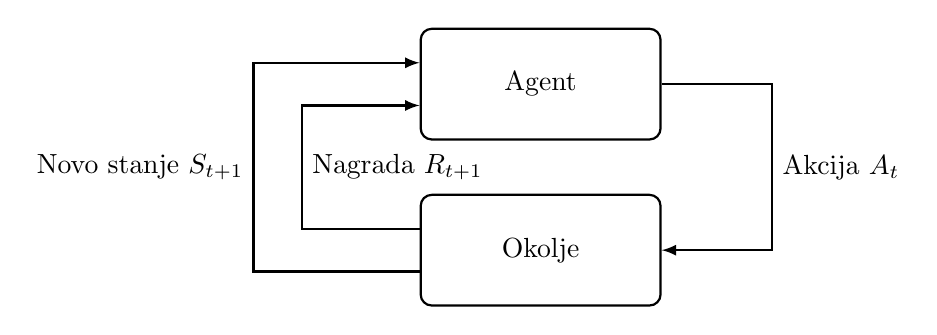
\begin{tikzpicture}[node distance = 6em, auto, thick]
            \node [block] (Agent) {Agent};
            \node [block, below of=Agent] (Okolje) {Okolje};
        
            \path [line] (Agent.0) --++ (4em,0em) |- node [near start]{Akcija $A_t$} (Okolje.0);
            \path [line] (Okolje.190) --++ (-6em,0em) |- node [near start] {Novo stanje  $S_{t+1}$} (Agent.170);
            \path [line] (Okolje.170) --++ (-4.25em,0em) |- node [near start, right] {Nagrada $R_{t+1}$} (Agent.190);
        \end{tikzpicture}
    \caption{Zanka spodbujevalnega učenja}
    \end{figure}
\end{center}
\subsubsection{Raziskovanje in izkoriščanje}
Eden izmed glavnih problemov, s katerim se srečamo pri spodbujevalnem učenju, je problem 
raziskovanja in izkoriščanja. Ko se agent uči, začne dojemati, katere akcije ali pa kombinacije 
akcij mu pripeljejo nagrado. Ko to ugotovi, seveda lahko začne te akcije \textit{izkoriščati} 
in prejemati vso nagrado, ki akcijam pripada. Pri tem pa naletimo na problem. Agent lahko izkorišča te 
akcije in nikoli ne ugotovi, da neka druga akcija prinese še višjo nagrado; tega ne izve, ker ne
\textit{raziskuje}. Če pa samo raziskuje, pa nikoli ne izkoristi potencialnih nagrad, ki jih sreča, 
torej se ničesar ne nauči. 

Uravnoteženje raziskovanja in izkoriščanja je pomemben problem, a se izkaže, da ima dokaj enostavno
rešitev (ki deluje dovolj dobro). Spoznali jo bomo v nadaljevanju.

\begin{zgled}[Raziskovanje v namiznih igrah]
    Pri namiznih igrah agent lahko odkrije strategijo, ki premaga določenega nasprotnika. To strategijo
    lahko potem izrablja in nasprotnika vedno premaga, ko pa naleti na drugega nasprotnika se lahko izkaže, 
    da je bila strategija učinkovita samo proti prvemu - naša strategija ni bila optimalna. Zato je 
    pomembno, da tudi ob odkritju dobre strategije agent še vedno raziskuje prostor strategij, to 
    najenostavneje dosežemo tako, da agenta prisilimo, da občasno igra naključne poteze.
\end{zgled}

Morda se nekaterim bralcem zdi, da smo zaenkrat preveč ">mahali z rokami"<. To je zato, ker želimo, 
da se do te točke razvije intuicija o predstavljenih pojmih. V nadaljevanju bomo do sedaj opisane 
stvari bolj formalizirali.


\subsection{Markovski proces odločanja}
Spomnimo se najprej procesa spodbujevalnega učenja in ga poskusimo opisati bolj formalno: 
imamo zaporedje časovnih korakov $t = 0, 1, 2, \dots$, ob katerih med sabo interaktirata agent 
in okolje. Ob koraku $t$ agent prejme od okolja stanje (oz. reprezentacijo stanja) $S_t \in 
\mathcal{S}$, kjer $\mathcal{S}$ označuje množico vseh stanj. Na podlagi stanja in strategije, 
ki jo ima, izbere akcijo $A_t \in \mathcal{A}(S_t)$, kjer $\mathcal{A}(S_t)$ predstavlja 
množico akcij, ki jih ima agent na voljo v stanju $S_t$. Rezultat te akcije je nagrada $R_{t+1} 
\in \mathcal{R}$, kjer $\mathcal{R}$ označuje množico vseh nagrad, in novo stanje $S_{t+1}$.

Čeprav se da vse opisane koncepte posplošiti na števne in celo neštevne množice stanj in akcij, 
se bomo mi omejili na končne množice. To je pri namiznih igrah dovolj.

\subsubsection{Markovska veriga}
Dogajanje pri spodbujevalnem učenju lahko v grobem opišemo z zaporedjem slučajnih spremenljivk $S_0,
S_1, \dots$ v diskretnem času, to je, s slučajnim procesom stanj $(S_t)_{t=0}^T$. Zato je pomembno, 
da si natančno pogledamo nekaj lastnosti, ki jih lahko pričakujemo. 

\begin{definicija}[Markovska veriga]
    Slučajni proces $(S_t)_{t=0}^T$ na končnem verjetnostnem prostoru 
    $(\Omega, \mathcal{F}, P)$ je \textbf{Markovska veriga} oz. \textbf{Markovski proces} (angl. 
    \textit{Markov chain}), če zanj velja Markovska lastnost
    $$
    P(S_{t+1} = s_{t+1}~|~S_{t} = s_{t}, \dots, S_0 = s_0) = P(S_{t+1} = s_{t+1}~|~S_{t} = s_{t}).
    $$
    Na kratko to \textit{prehodno verjetnost} označimo $p_{ss'} := P(S_{t+1} = s'~|~S_{t} = s)$.
    Opazimo, da lahko te verjetnsoti zložimo v matriko $\mathcal{P} := 
    [p_{ss'}]_{s,s'\in \mathcal{S} }$, ki ji pravimo \textit{prehodna matrika}.

    Zdaj Markovsko verigo predstavimo še na alternativni način: kot dvojico $(\mathcal{S}, 
    \mathcal{P})$, kjer je $\mathcal{P}$ zgoraj definirana prehodna matrika, $\mathcal{S}$ pa 
    množica vseh stanj.
\end{definicija}

Markovska lastnost pomeni, da je prihodnost neodvisna od preteklosti, če poznamo sedanjost. 
Spodbujevalno učenje se ukvarja predvsem s problemi, kjer to dejstvo drži. Tudi pri našem 
ciljnem problemu to načeloma velja: če pogledamo igralno ploščo na katerikoli točki, pogosto 
izvemo enako o trenutnem stanju, kot če bi opazovali igro od začetka.

\subsubsection{Markovski proces nagrajevanja}
Podoben koncept, ki se malo bolj približa dejanski situaciji v spodbujevalnem učenju, je
\textit{Markovski proces nagrajevanja}. Kot že ime morda namigne, je precej podoben Markovski 
verigi, le da v njem nastopajo \textit{nagrade}. 

\begin{definicija}[Markovski proces nagrajevanja]
    Pričakovani nagradi glede na stanje $s$ pravimo \textbf{nagradna funkcija} (angl. \textit{reward 
    function}) in jo označimo
    $$
    \mathcal{R}_s = E[R_{t+1}~|~S_{t} = s].
    $$
    Naboru $(\mathcal{S}, \mathcal{P}, \mathcal{R}, \gamma)$, za katerega velja
    \begin{itemize}
        \item $\mathcal{S}$ je (končna) množica stanj,
        \item $\mathcal{P}$ je prehodna matrika $\mathcal{P}_{ss'} = P(S_{t+1} = s'~|~S_{t} = s)$, 
        \item $\mathcal{R}$ je \textit{nagradna funkcija} 
                $\mathcal{R}_s = \mathrm{E}[R_{t+1}~|~S_{t} = s]$, 
        \item $\gamma \in [0,1]$ je \textit{diskontni faktor}, 
    \end{itemize}
    pravimo \textbf{Markovski proces nagrajevanja} (angl. \textit{Markov reward process}).
\end{definicija}

Od navadne Markovske verige se torej razlikuje samo v prisotnosti nagrad ob vsakem koraku. Če te 
nagrade postavimo na $R_t = 0$ za vsak $t$, dobimo navadno Markovsko verigo. Pomembna razlika je še 
prisotnost diskontnega faktorja $\gamma$. Če velja $\gamma < 1$, potem procesu pravimo \textit{
diskontirani Markovski proces nagrajevanja}.

Diskontiranje je motivirano iz različnih vidikov: po eni strani nam pomaga, da se v primeru 
cikličnih procesov izognemo neomejenim povračilom. Poleg tega pa je diskontiranje v mnogo pogledih 
naraven način za opis situacije: pogosto imamo raje nagrade, ki pridejo prej. Primer tega poznamo 
recimo iz ekonomije; denar, ki ga dobimo kasneje nam pomeni manj, kot tisti, ki ga dobimo takoj. 

Še vedno pa tovrsten proces ne opiše situacije, v kateri se znajdemo pri spodbujevalnem učenju, saj 
ne vsebuje koncepta akcij. Je pa že dovolj ">globok"<, da v njem lahko definiramo vrednostno 
funkcijo $v(s) = \mathrm{E} [G_t~|~S_t = s]$, ki je v tem primeru neodvisna od strategije $\pi$, 
saj strategija v tem modelu nima pomena. 

Za vrednostno funkcijo lahko izpeljemo rekurzivno enačbo, s pomočjo katere lahko ">rešimo"< Markovski
proces nagrajevanja. S tem mislimo, da vsakemu stanju dodelimo pravo vrednost. To je vrednost, ki jo 
stanju določata nagrada in nagradna funkcija.

\begin{align*}
    v(s) &= \mathrm{E} [G_t~|~S_t = s] \\
         &= \mathrm{E} [\sum_{k=0}^\infty \gamma^k R_{t + k + 1}~|~S_t = s] \\
         &= \mathrm{E} [R_{t+1} + \sum_{k=1}^\infty \gamma^k R_{t + k + 1}~|~S_t = s] \\
         &= \mathrm{E} [R_{t+1} + \gamma(\sum_{k=1}^\infty \gamma^{k-1} R_{t + k + 1})~|~S_t = s] \\
         &= \mathrm{E} [R_{t+1} + \gamma G_{t+1}~|~S_t = s] \\
         &= \mathrm{E} [R_{t+1} + \gamma v(S_{t+1})~|~S_t = s].
\end{align*}

Dobili smo torej 
$$
v(s) = \mathrm{E} [R_{t+1} + \gamma v(S_{t+1})~|~S_t = s]
$$
oziroma 
\begin{equation}\label{beMRP}
    v(s) = \mathcal{R}_s + \gamma \sum_{s' \in \mathcal{S}} \mathcal{P}_{ss'} v(s'),
\end{equation} 
kjer smo upoštevali aditivnost in idempotentnost pogojnega matematičnega upanja. Enačba \eqref{beMRP}
je \textbf{Bellmanova enačba za Markovkse procese nagrajevanja}.

Ker se ukvarjamo s primerom, ko je stanj končno mnogo, recimo $n$, jih lahko brez škode za 
splošnost označimo kar $1, \dots, n$. Potem lahko Bellmanovo enačbo prepišemo v matrični obliki
\begin{align*}
    \begin{bmatrix}
        v(1) \\ 
        \vdots \\ 
        v(n)
    \end{bmatrix}
    &=
    \begin{bmatrix}
        \mathcal{R}_1 \\ 
        \vdots \\ 
        \mathcal{R}_n 
    \end{bmatrix}
    + \gamma
    \begin{bmatrix}
        \mathcal{P}_{11} \dots \mathcal{P}_{1n} \\ 
        \vdots \\ 
        \mathcal{P}_{n1} \dots \mathcal{P}_{nn}
    \end{bmatrix}
    \begin{bmatrix}
        v(1) \\ 
        \vdots \\ 
        v(n)
    \end{bmatrix} \\
    \intertext{ali krajše}
    v &= \mathcal{R} + \gamma \mathcal{P}v.
\end{align*}
Opazimo, da je to \textit{linearna} enačba, ki jo lahko eksplicitno rešimo: 
\begin{align*}
    v &= \mathcal{R} + \gamma \mathcal{P}v \\
    (I - \gamma \mathcal{P}) v &= \mathcal{R} \\
    v &= (I - \gamma \mathcal{P})^{-1} \mathcal{R}.
\end{align*}
Ta rešitev predpostavlja obrnljivost matrike $(I - \gamma \mathcal{P})$ in računanje njenega 
inverza, kar zahteva $O(n^3)$ operacij, zato je smiselna samo za majhne procese. Za večje 
obstajajo iterativni algoritmi in metode, nekatere izmed njih bomo spoznali v naslednjem odseku.

TA DEL LAHKO MATEMATIZIRAŠ - ENOLIČNOST REŠITEV

\subsubsection{Markovski proces odločanja}
Kot ime že nakazuje, \textbf{Markovski proces odločanja} (angl. \textit{Markov decision process (MDP)}) 
razširja koncept procesa nagrajevanja z dodatkom odločanja - akcij. S tem dodatkom imamo v popolnosti 
opisan problem spodbujevalnega učenja: proučujemo torej nek proces, kjer ima agent možnost odločanja, 
izid pa je vsaj delno slučajen in odvisen od okolja. 

\begin{opomba}
    Ker v Markovskem procesu odločanja nastopajo (in imajo poglavitno) vlogo akcije, seveda pomembno 
    vplivajo na nagradno funkcijo in prehodno matriko, zato moramo ta koncepta ustrezno prilagoditi:
    \begin{align*}
    \mathcal{R}_s^a &= E[R_{t+1}~|~S_{t} = s, A_t = a], \\
    \mathcal{P}_{ss'}^a &= P(S_{t+1} = s'~|~S_t = s, A_t = a)
    \end{align*}
\end{opomba}

\begin{definicija}[Markovski proces odločanja]
    Naboru $(\mathcal{S}, \mathcal{A}, \mathcal{P}, \mathcal{R}, \gamma)$, za katerega velja
    \begin{itemize}
        \item $\mathcal{S}$ je (končna) množica stanj,
        \item $\mathcal{A}$ je (končna) množica akcij, 
        \item $\mathcal{P}$ je prehodna matrika $\mathcal{P}_{ss'}^a = P(S_{t+1} = s'~|~
                S_t = s, A_t = a)$, 
        \item $\mathcal{R}$ je \textit{nagradna funkcija} 
                $\mathcal{R}_s^a = \mathrm{E}[R_{t+1}~|~S_{t} = s, A_t = a]$, 
        \item $\gamma \in [0,1]$ je \textit{diskontni faktor}, 
    \end{itemize}
    pravimo \textbf{Markovski proces odločanja} (angl. \textit{Markov decision process}).
\end{definicija}

V kontekstu MDP-jev lahko sedaj formalno definiramo strategijo agenta $\pi$, ki je zahvaljujoč 
Markovski lastnosti odvisna od enega (trenutnega) stanja in ne od celotne zgodovine procesa. 
Definiramo tudi vrednostno funkcijo stanja $v_{\pi}(s)$ in vrednostno funkcijo akcije $q_{\pi}(s, a)$. 
Njihove definicije se ne spremenijo, so pa sedaj formalno vmeščene v model.

Opazimo, da je v MDP-ju pri fiksni strategiji $\pi$ zaporedje oz. proces stanj $S_1, S_2, \dots$ 
Markovska veriga $(\mathcal{S}, \mathcal{P}^\pi)$. Če v zaporedje stanj pomešamo še nagrade, 
torej $S_1, R_2, S_2, R_3, \dots$, dobimo Markovski proces nagrajevanja $(\mathcal{S}, 
\mathcal{P}^\pi, \mathcal{R}^\pi, \gamma)$, kjer smo označili

\begin{align*}
    \mathcal{P}^\pi &= \sum_{a \in \mathcal{A}} \pi(a|s) \mathcal{P}_{ss'}^a \\
    \mathcal{R}^\pi &= \sum_{a \in \mathcal{A}} \pi(a|s) \mathcal{R}_{s}^a. 
    \end{align*}

\begin{opomba}
    Morda je nekatere bralce zbodlo, da v zaporedju stanj in nagrad $S_1$ ne sledi $R_1$, temveč 
    $R_2$. Za tako notacijo smo se odločili, da poudarimo, da okolje agentu sočasno poda stanje $S_2$
    in nagrado $R_2$, glede na stanje $S_1$ pa se agent odloča o akciji $A_1$.
\end{opomba}

MDP-ji so splošna orodja za obravnavo stohastičnih procesov, ki vključujejo odločitve v diskretnem 
času. Njihov utemeljitelj je Richard Bellman, ki je znan predvsem po izumu dinamičnega 
programiranja, zato morda ni presenetljivo, da nam prav dinamično programiranje poda osnovo za 
njihovo reševanje.
Kot pri procesih nagrajevanja, lahko tudi tu izpeljemo Bellmanovo enačbo. Na popolnoma enak način 
kot pri procesih nagrajevanja lahko izpeljemo rekurzivni  
\begin{align*}
    v_\pi(s) &= \mathrm{E} [R_{t+1} + \gamma v_\pi(S_{t+1})~|~S_t = s], \\
    q_\pi(s, a) &= \mathrm{E} [R_{t+1} + \gamma q_\pi(S_{t+1}, A_{t+1})~|~S_t = s, A_t = a].
\end{align*}
Opazimo, da $v_\pi$ in $q_\pi$ povezujta zvezi
\begin{align*}
    v_\pi(s) &= \sum_{a \in \mathcal{A}} \pi(a|s)q_\pi(s, a), \\
    q_\pi(s, a) &= \mathcal{R}_s^a + \gamma \sum_{s' \in \mathcal{S}} \mathcal{P}_{ss'}^a v_\pi(s').
\end{align*}

Smiselno se zdi, da bi se vsota $q_\pi(s, a)$ po akcijah, uteženo z ustreznimi verjetnostmi izbire 
posamezne akcije v stanju $s$ $\pi(a|s)$ seštela v $v_\pi(s)$ in tudi res je tako, saj
\begin{align*}
    v_\pi(s) &= \mathrm{E} [G_t~|~S_t = s] \\
\end{align*}










Če zvezi združimo, dobimo

\begin{align}
    v_\pi(s) &= \sum_{a \in \mathcal{A}} \pi(a|s) \left[\mathcal{R}_s^a + 
    \gamma \sum_{s' \in \mathcal{S}} \mathcal{P}_{ss'}^a v_\pi(s') \right], \label{bepMDP} \\
    q_\pi(s, a) &= \mathcal{R}_s^a + \gamma \sum_{s' \in \mathcal{S}} 
    \mathcal{P}_{ss'}^a \left[\sum_{a' \in \mathcal{A}} \pi(a'|s')q_\pi(s', a') \right].
\end{align}
Enačbo \eqref{bepMDP} imenujemo \textbf{Bellmanova enačba pričakovanja} (angl. \textit{Bellman 
expectation equation}), ki ima ponovno matrično obliko in eksplicitno (ENOLIČNO - ZAKAJ, TU 
DODATNA RAZLAGA) rešitev: 
\begin{align*}
    v_\pi &= \mathcal{R}^\pi + \gamma \mathcal{P}^\pi v_\pi \\
    v_\pi &= (I - \gamma \mathcal{P}^\pi)^{-1} \mathcal{R}^\pi
\end{align*}

Ta enačba je sicer pomembna, a določi samo prave vrednosti glede na neko strategijo. Nas pa zanima 
">rešitev"< MDP-ja. To pomeni, da želimo najti strategijo, ki nam bo prinesla največjo nagrado.

\subsubsection{Optimalne vrednostne funkcije}
\begin{definicija}
    ~
    \begin{itemize}
        \item \textbf{Optimalna vrednostna funkcija stanja} (angl. \textit{optimal state-value 
                function}) $v_*(s)$ je vrednostna funkcija za strategijo, ki vrne največje vrednosti
                $$
                v_*(s) = \max_\pi v_\pi(s).
                $$
        \item \textbf{Optimalna vrednostna funkcija akcije} (angl. \textit{optimal action-value 
                function}) $q_*(s, a)$ je analog optimalni vrednostni funkciji stanja
                $$
                q_*(s, a) = \max_\pi q_\pi(s, a).
                $$
        \item Na množici vseh možnih strategij $\Pi$ definiramo delno urejenost na naslednji način:
                $$
                \pi \geq \pi', \medspace \text{če } v_\pi(s) \geq v_{\pi'}(s) ~ \forall s. 
                $$
                Če za strategiji velja kot zgoraj, pravimo, da je $\pi$ \textit{boljša ali enaka} 
                kot $\pi'$.
        \item \textbf{Optimalna strategija} je strategija $\pi_*$, ki je boljša ali enaka od vseh 
                ostalih strategij $\pi \in \Pi$.
    \end{itemize}
\end{definicija}
Sedaj lahko uporabimo naslenji izrek.

\begin{izrek}\label{optim}
    Za vsak Markovski proces odločanja velja: 
    \begin{itemize}
        \item Obstaja \textit{optimalna} strategija $\pi_*$, ki je boljša ali enaka kot vse ostale 
                strategije; $\pi_* \geq \pi \text{ } \forall \pi \in \Pi$. 
        
        \item Vedno obstaja \textit{deterministična} optimalna strategija $\pi: \mathcal{S} 
                \rightarrow \mathcal{A}$. 
        \item Vse optimalne strategije določajo enako optimalno vrednostno funkcijo stanja in 
                optimalno vrednostno funkcijo akcije; 
                \begin{align*}
                    v_{\pi*}(s) &= v_*(s) \\
                    q_{\pi*}(s, a) &= q_*(s, a).
                \end{align*}
    \end{itemize} 
\end{izrek}

OPOMBA: SKLIC NA DOKAZ

Izrek nam pove, da če poznamo $q_*(s, a)$, poznamo tudi optimalno deterministično strategijo, 
ki jo dobimo kot $\pi_*(a|s) = \mathbbm{1} (a =\text{arg}\max_{a \in \mathcal{A}} q_*(s, a))$.

Podobno kot za poljubne vrednostne funkcije, lahko tudi za optimalne vrednostne funkcije 
izpeljemo Bellmanovo enačbo, ki jo sedaj imenujemo \textbf{Bellmanova enačba optimalnosti} (angl. 
\textit{Bellman optimality equation}). Sprva opazimo, da $q_*$ in $v_*$ povezujeta enaki zvezi kot 
$q_\pi$ in $v_\pi$:
\begin{align*}
    v_*(s) &= \max_a q_*(s, a), \\
    q_*(s, a) &= \mathcal{R}_s^a + \gamma \sum_{s' \in \mathcal{S}} \mathcal{P}_{ss'}^a v_*(s).
\end{align*}
Ti zvezi nato vstavimo eno v drugo, in dobimo enačbi: 

\begin{align}\label{beo}
    v_*(s) &= \max_a \mathcal{R}_s^a + \gamma \sum_{s' \in \mathcal{S}} \mathcal{P}_{ss'}^a v_*(s), \\
    q_*(s, a) &= \mathcal{R}_s^a + 
                \gamma \sum_{s' \in \mathcal{S}} \mathcal{P}_{ss'}^a \max_{a'} q_*(s', a').
\end{align}
Opazimo, da sta enačbi tokrat nelinearni, kar močno oteži direktno reševanje. Na srečo pa tudi 
v tem primeru pridejo prav metode iz naslednjega odseka.

MALO BOLJ NATANČNO O TEM KAKO DO OPT STRAT IZ FUNKCIJE, DOKAZI, IZPELJAVE, ...

\section{Algoritmi pri spodbujevalnem učenju}
\label{algoritmi}
Algoritmov za reševanje MDP-jev je precej. Mi se bomo omejili predvsem na algoritme, ki se učijo 
prek vrednostne funkcije in izhajajo iz dinamičnega programiranja, a naj na tem mestu omenimo, 
da obstajajo tudi algoritmi, ki posodabljajo strategijo neposredno (MOGOČE KAKŠEN REFERENCE ALI 
PA KEJ).

Izjemnega pomena pri reševanju je dejstvo, ali je znana matrika $\mathcal{P}$ in nagradna funkcija 
$\mathcal{R}_s^a$. Izkaže se, da je večina problemov takih, da ti dve stvari nista znani. Eden izmed 
takih problemov je tudi igranje namiznih iger -- ne poznamo strategije našega nasprotnika, zato ne 
poznamo verjetnosti prehodov med stanji.

Poleg tega naj na tem mestu omenimo, da reševanju celotnega problema spodbujevalnega učenja 
pravimo \textbf{načrtovanje} (angl. \textit{planning}), le-ta pa se deli na dve stopnji: 

\begin{itemize}
    \item \textbf{Napovedovanje} - pri tem podproblemu podamo nek MDP in strategijo, algoritem nam 
            vrne vrednostno funkcijo stanja (glede na strategijo).   
    \item \textbf{Upravljanje} - to je bolj poln problem: podan je MDP, algoritem pa nam vrne 
            optimalno vrednostno funkcijo in pripadajočo optimalno strategijo.
\end{itemize}

\subsection{Dinamično programiranje - reševanje poznanih MDP-jev}
Dinamično programiranje je optimizacijska metoda, ki deluje na principu deljenja velikega problema 
na manjše prekrivajoče podprobleme. V jedru reševanja je \textbf{Bellmanova enačba}, ki opisuje 
odnos med vrednostmi podproblemov in vrednostjo glavnega problema. Ker je idejo dinamičnega 
programiranja (DP) in MDP-jev dobil Bellman ob istem času, je naravno, da je DP metoda, ki je 
prilagojena prav situaciji v MDP-ju.

Problem mora v splošnem zadoščati dvema lastnostima, da je zanj primerno reševanje z dinamičnim 
programiranjem. Prvi pravimo \textbf{lastnost optimalne podstrukture}, ki pravi, da lahko problem 
razstavimo na podprobleme in rešitve podproblemov lahko potem sestavimo nazaj v rešitev celotnega 
problema. Druga pomembna lastnost pa so \textbf{prekrivajoči podproblemi}, ki implicira, da lahko 
že poznane rešitve podproblemov večkrat uporabimo.

Opazimo, da obe lastnosti veljata za MDP-je; Bellmanova enačba, nam razdeli problem na 
podprobleme, vrednostna funkcija pa hrani in ponovno uporablja rešitve. Lastnosti veljata tudi 
za Markovske procese nagrajevanja, zato lahko metode, ki jih bomo spoznali, uporabimo za reševanje
tovrstnih procesov. Nam je seveda v interesu reševati MDP-je, zato se bomo posvetili temu.

(MORDA BOLJ FORMALNO O BELLMANOVIH ENAČBAH - NI TREBA?)

\subsubsection{Iterativno ocenjevanje strategije}
Algoritem deluje na MDP-ju, katerega prehodna matrika je znan podatek. Poleg tega potrebuje tudi 
fiksno strategijo $\pi$. Algoritem torej rešuje zgorlj parcialni problem, to je problem 
napovedovanja. V ozadju je glavna ideja Bellmanova enačba pričakovanja, z njo na vsakem koraku 
posodobimo $v_k(s)$ v $v_{k+1}(s)$ s pomočjo $v(s')$, kjer je $s'$
naslednje stanje od $s$. Enačba iteracije se potem glasi 
\begin{align*}
    v_{k+1}(s) &= \sum_{a \in \mathcal{A}} \pi(a|s) \left[ \mathcal{R}_s^a + 
        \gamma \sum_{s' \in \mathcal{S}} \mathcal{P}_{ss'}^a v_k(s') \right] \text{ ali na kratko}\\
    v_{k+1} &= \mathcal{R}^\pi + \gamma \mathcal{P}^\pi v_k.
\end{align*}

\begin{izrek}\label{ios}
    Iterativno ocenjevanje strategije konvergira proti vrednostni funkciji, ki jo določa strategija 
    $\pi$.
\end{izrek}

Izrek bomo dokazali samo v primeru končnih MDP-jev, to pomeni, da je prostor stanj $\mathcal{S}$ 
končen, torej $|\mathcal{S}| < \infty$. V tem primeru je prostor vrednostnih funkcij $\mathcal{V}$
vektorski prostor. Vsaka točka v njem korespondira z eno vrednostno funkcijo $v(s)$.

\begin{definicija}[Neskončna norma za vrednostne funkcije]
    Je norma, ki meri ">razdaljo"< med vrednostnima funkcijama $v$ in $u$. Izračunamo jo kot 
    največjo razliko med vrednosti stanj oz. 
    $$
    ||v - u||_\infty = \max_{s \in \mathcal{S}} |v(s) - u(s)|.
    $$
\end{definicija}

\begin{proof}[Dokaz izreka \ref{ios}]
    Pokazali bomo, da iz iteracije lahko pridobimo skrčitev, iz Banachovega izreka o fiksni točki 
    potem sledi naš rezultat.
    Definiramo \textbf{Bellmanov operator pričakovanja} kot 
    $$
    T_\pi(v) = \mathcal{R}_\pi + \gamma \mathcal{P}_\pi v.
    $$
    Naj bosta $u$ in $v$ vrednostni funkciji. Potem je zgornji operator skrčitev glede na neskončno 
    normo: 
    \begin{align*}
        ||T_\pi(v) - T_\pi(u)||_\infty &= ||\mathcal{R}_\pi + \gamma \mathcal{P}_\pi v - 
                                            \mathcal{R}_\pi + \gamma \mathcal{P}_\pi u||_\infty \\  
        &= ||\gamma \mathcal{P}_\pi (v - u)||_\infty \\
        &\leq ||\gamma \mathcal{P}_\pi||_\infty ||v - u||_\infty \\
        &\leq \gamma ||v - u||_\infty,
    \end{align*}
    kjer smo upoštevali, da velja $||\mathcal{P}_\pi||_\infty \leq 1$, saj so elementi 
    $\mathcal{P}_\pi$ verjetnosti. Po Bellmanovi enačbi pričakovanja je $v_\pi$ fiksna točka 
    za $T_\pi$, rezultat nato sledi iz Banachovega izreka.
\end{proof}

S tem procesom tako res dobimo vrednostno funkcijo, ki jo določa strategija, a strategija je 
statična; to reši problem napovedovanja. 

Da rešimo problem upravljanja, uporabimo enostavno idejo: strategijo izboljšamo \textbf{požrešno}. 
To pomeni, da izberemo tako akcijo, ki nas pripelje v stanje $s$, ki je dosegljivo in ima največjo 
vrednost $v_\pi(s)$. Na vsakem koraku torej izberemo največjo vrednost ne glede na vse, od tu pride 
ime \textit{požrešno}.

\subsubsection{Iteracija strategije}
Algoritem, ki ga dobimo s tem, da združimo iterativno ocenjevanje strategije in požrešno izboljšavo 
strategije, imenujemo iteracija strategije (angl. \textit{policy iteration}). S tem algoritmom 
lahko sedaj rešimo problem upravljanja in s tem celoten problem poznanega MDP-ja. V praksi to pomeni, 
da začnemo z naključno strategijo, jo iterativno ocenimo, nato na podlagi rezultata požrešno izboljšamo 
strategijo in ta dva koraka ponavljamo.

\begin{izrek}
    Iteracija strategije vedno konvergira k optimalni strategiji $\pi_*$.
\end{izrek}

\begin{proof}
    Ukvarjali se bomo samo z determinističnimi strategijami, saj so zaradi požrešne izbire 
    strategije le-te vedno deterministične, razen začetne. Ker je izbira začetne strategije za 
    trditev nepomembna, lahko izberemo neko naključno deterministično strategijo $a = \pi(s)$.

    Požrešno vedenje zdaj za nas pomeni, da vzamemo $\pi'(s) = 
    \text{arg}\max_{a \in \mathcal{A}} q_\pi(s, a)$. To očitno izboljša vrednost za vsako stanje 
    $$
    q_\pi(s, \pi'(s)) = \max_{a \in \mathcal{A}} q_\pi(s, a) \geq q_\pi(s, \pi(s)) = v_\pi(s).
    $$
    Posledično izboljša tudi vrednostno funkcijo: 
    \begin{align*}
        v_\pi(s) &\leq q_\pi(s, \pi'(s)) = \mathrm{E}_{\pi'} [R_{t+1} + 
            \gamma v_\pi(S_{t+1})~|~S_t = s] \\
        &\leq \mathrm{E}_{\pi'} [R_{t+1} + \gamma q_\pi(S_{t+1} \pi'(S_{t+1}))~|~S_t = s] \\
        &\leq \mathrm{E}_{\pi'} [R_{t+1} + \gamma R_{t+2} + 
            \gamma^2 q_\pi(S_{t+2} \pi'(S_{t+2}))~|~S_t = s] \\
        &\leq \mathrm{E}_{\pi'} [R_{t+1} + \gamma R_{t+2} + \dots~|~S_t = s] = v_{\pi'}(s).
    \end{align*}

Če vrednost preneha rasti, dobimo 
$$
q_\pi(s, \pi'(s)) = \max_{a \in \mathcal{A}} q_\pi(s, a) = q_\pi(s, \pi(s)) = v_\pi(s).
$$
To se zgodi, saj zaradi končnih nagrad tudi vrednostne funkcije zavzemajo končne vrednosti. 
Potem opazimo, da je zaradi $v_\pi(s) = \max_{a \in \mathcal{A}} q_\pi(s, a)$ zadoščeno Bellmanovi 
enačbi optimalnosti in zato po izreku \ref{optim} velja $v_\pi(s) = 
v_*(s) \text{ } \forall s \in \mathcal{S}$, torej je $\pi$ optimalna strategija.
\end{proof}

\subsubsection{Iteracija vrednosti}
K problemu lahko pristopimo tudi neposredno prek Bellmanove enačbe optimalnosti in se s tem 
izognemo neposredni uporabi strategije, vseeno pa rešimo problem upravljanja. Ideja je podobna kot 
pri iterativnem ocenjevanju strategije, le da imamo drugačno enačbo za iteracijo: 
\begin{align*}
    v_{k+1}(s) &= \max_{a \in \mathcal{A}} \left[ \mathcal{R}_s^a + 
        \gamma \sum_{s' \in \mathcal{S}} \mathcal{P}_{ss'}^a v_k(s') \right] \\
    \intertext{oziroma}
    v_{k+1} &= \max_{a \in \mathcal{A}} \mathcal{R}^a + \gamma \mathcal{P}^a v_k.
\end{align*}
Podobno kot pri iterativnem ocenjevanju strategije pokažemo, da zgornja iteracija konvergira k 
$v_*$.

\subsubsection{Časovna zahtevnost}
Za korak obeh iteracij je potrebnih $O(mn^2)$ operacij, kjer je $m$ število akcij in $n$ število 
stanj. Popolnoma enake algoritme lahko uporabimo za iteracijo $q_\pi(s, a)$ oz. $q_*(s, a)$, le 
da sedaj pridemo do časovne zahtevnosti $O(m^2n^2)$.

\subsection{Monte Carlo}
Do sedaj smo se ukvarjali s poznanim MDP-jem, kar pa ni naš končen cilj. V nadaljevanju se bomo 
posvetili nepoznanim. Metode, ki jih bomo spoznali so tako bolj splošno aplikativne, svoje 
bistvo pa črpajo pri do sedaj poznanem.

Prva taka metoda je Monte Carlo. Spopada se s problemom \textit{napovedovanja} z dodatno izboljšavo, 
da ne rabi poznati matrike $\mathcal{P}$. Potrebujemo pa strategijo $\pi$, na podlagi katere opazujemo
epizode dogajanja. Ideja delovanja je, da se namesto na direktno računanje pričakovanega povračila
$G_t = \sum_{k=0}^\infty \gamma^k R_{t + k + 1}$, osredotočimo na računanje \textit{empiričnega} 
povračila. To storimo tako, da za vsako stanje $s$ definiramo števec $N(s)$, ki beleži, kolikokrat 
je bilo stanje obiskano. Ta števec ne beleži zgolj obiskov znotraj epizode, temveč skozi celoten 
proces učenja. Za vsako stanje hranimo še $S(s)$, ki ga posodobimo za vsa stanja na koncu epizode
tako, da prištejemo dejansko opaženo empirično povračilo $G_t$, ki pripada posameznemu stanju.
Po koncu učenja enostavno za vsako stanje delimo $S(s)$ z $N(s)$ in tako dobimo vzorčno povprečje za 
dejanski $v(s)$.
\begin{itemize}
    \item Ob vsakem (ali samo prvem) obisku stanja $s$: 
        \begin{align*}
            N(s) &\leftarrow N(s) + 1 \\
            S(s) &\leftarrow S(s) + G_t.
        \end{align*}
    \item Po zadostni količini epizod (ob koncu učenja): 
        $$
        V(s) \leftarrow S(s) / N(s)
        $$
\end{itemize}

TOLE MALO BOLJ RAZDELAJ - MONTE CARLO IMA KVADRATIČNO KONVERGENCO, SUTTON BARTO, RAZLOŽI KAJ JE 
PUŠČICA

Opazimo, da vrednost $V(s)$ konvergira proti $v_\pi(s)$, ko gre $N(s) \rightarrow \infty$ po 
krepkem zakonu velikih števil. Opazimo tudi, da metoda deluje samo za probleme, ki imajo končne 
epizode, saj šele takrat lahko poznamo $G_t$. Če za vsako stanje $s$ hranimo $N(s)$ in $S(s)$, 
tako dobimo oceno za $v_\pi(s)$ za vsak $s \in \mathcal{S}$.

Prostorsko zahtevnost lahko izboljšamo, če upoštevamo, da povprečje $\mu$ nekega zaporedja slučajnih 
spremenljivk $X_1, X_2, \dots$ izračunamo inkrementalno:
\begin{align*}
    \mu_k &= \frac{1}{k} \sum_{i = 1}^k X_i \\
        &= \frac{1}{k} \left[X_k + \sum_{i = 1}^{k-1} X_i \right] \\
        &= \frac{1}{k} \left[X_k + (k-1) \mu_{k-1} \right] \\
        &= \mu_{k-1} + \frac{1}{k} \left(X_k - \mu_{k-1} \right).
\end{align*}
Na podlagi te zveze lahko implementiramo inkrementalni Monte Carlo, tako da po končani epizodi 
za vsako stanje $S_t$ s povračilom $G_t$ posodobimo (ODLOČI SE ZA $S_t$ ALI s): 

\begin{align*}
    N(S_t) &\leftarrow N(S_t) + 1, \\
    V(S_t) &\leftarrow V(S_t) + \frac{1}{N(S_t)} (G_t - V(S_t)).
\end{align*}
Izkaže se, da lahko zgornje še malo posplošimo in namesto faktorja $1/N(S_t)$ uporabimo splošni 
faktor $\alpha$
\begin{equation}\label{mc}
    V(S_t) \leftarrow V(S_t) + \alpha (G_t - V(S_t)),
\end{equation}
kjer $\alpha$ imenujemo \textbf{velikost koraka} oz. \textbf{hitrost učenja} (angl. 
\textit{learning rate}). Posodobitveno pravilo \eqref{mc} je konkreten primer bistvene ideje 
spodbujevalnega učenja prek vrednostne funkcije. Vsi ostali algoritmi nam dajo pravilo podobne 
oblike: 
\begin{equation}\label{osnova}
    \textit{nova ocena} \leftarrow \textit{stara ocena} + \textit{korak } 
    (\textit{tarča} - \textit{stara ocena}).
\end{equation}

\subsection{Algoritem TD($0$)}
V spodbujevalnem učenju obstaja skupina algoritmov, ki se imenujejo \textbf{algoritmi učenja s 
časovno razliko} (angl. \textit{temporal-difference learning}). Delujejo v podobnih pogojih kot 
Monte Carlo in tudi dosegajo enak cilj. Pomembna razlika je, da ne potrebujejo empiričnega povračila 
pri posodobitvi. Zaradi tega lahko delujejo tudi v sistemih, ki se ne delijo na epizode oz. ne 
potrebujejo končanih epizod za svoje delovanje.

Najpreprostejši algoritem učenja s časovno razliko je TD($0$). Ideja je, da v stanju ocenimo
povračilo kot $G_t \approx R_{t+1} + \gamma V(S_{t+1}).$ To potem uporabimo za \textit{tarčo}
v pravilu \eqref{osnova}. To nam da pravilo
\begin{equation}
    V(S_t) \leftarrow V(S_t) + \alpha (R_{t+1} + \gamma V(S_{t+1}) - V(S_t)).
\end{equation}
Iz tega zelo hitro ugotovimo, od kod pride poimenovanje. Algoritem za svoje posodabljanje uporablja 
podatek iz naslednjega trenutka -- torej se uči s časovno razliko. Pomembno je omeniti tudi, da za 
učenje uporablja oceno vrednosti naslednjega stanja, torej ocenjuje na podalgi ocene. Temu pravimo 
\textit{zankanje} (angl. \textit{bootstrapping}).

\subsubsection{Primerjava z Monte Carlo}
\begin{itemize}
    \item Tarča pri MC je nepristranska ocena $v_\pi(S_t)$, medtem ko je pri TD($0$) tarča 
    pristranska ocena. Ta prednost MC je uravnotežena s tem, da ima tarča pri TD($0$) nižjo varianco, 
    saj je odvisna od ene same slučajne spremenljivke, medtem ko je pri MC odvisna od mnogih 
    slučajnih dogodkov.
    
    \item Prav tako je pomembna razlika v dejstvu, da MC nujno rabi popolne epizode in se lahko
    izvede le po končani epizodi, TD($0$) pa se lahko uči sproti (angl. \textit{online}) in sploh 
    ne potrebuje končnih epizod. Seveda pa lahko TD($0$) uporabimo tudi za učenje samo ob koncu 
    posameznih epizod (angl. \textit{offline}).

    \item Razlika je tudi v tem, kam konvergirata algoritma, če imamo na voljo samo končno 
    količino epizod. Naj $K$ označuje število epizod in $k$ nakazuje, v kateri epizodi smo. Potem 
    MC konvergira k rešitvi z minimalno povprečno kvadratno napako (MSE) 
    $$
    \sum_{k=1}^K \sum_{t=1}^{T_k} (G_t^k - V(s_t^k))^2,
    $$
    torej se najbolje prilega opazovanim povračilom. TD($0$) pa konvergira k rešitvi modela največjega 
    verjetja Markova; to je rešitev MDP-ja, ki se najbolje prilega podatkom. Dobimo torej naslednji 
    cenilki: (TO SI ŠE POGLEJ)
    \begin{align*}
        \hat{\mathcal{P}}_{ss'}^a &= \frac{1}{N(s, a)} \sum_{k=1}^K \sum_{t=1}^{T_k} 
                \mathbbm{1}(s_t^k, a_t^k, s_{t+1}^k = s, a, s') \\
        \hat{\mathcal{R}}_{s}^a &= \frac{1}{N(s, a)} \sum_{k=1}^K \sum_{t=1}^{T_k} 
                \mathbbm{1}(s_t^k, a_t^k = s, a)r_t^k
    \end{align*}

    \item Zadnja pomembna razlika je, da TD izrabi Markovsko lastnost, medtem ko je MC ne. Zato je 
    vsaj v teoriji TD veliko bolj učinkovit v MDP-jih.
\end{itemize}

\begin{zgled}[Ti si sodnik - IZ SUTTON BARTO UČBENIKA]
    Recimo, da imamo na voljo za učenje naslednjih 8 epizod: 
    A $0$, B, $0$;
    B $1$;
    B $1$;
    B $1$;
    B $1$;
    B $1$;
    B $1$;
    B $0$

    To pomeni recimo, da smo prvo epizodo začeli v stanju A, nato dobili nagrado $0$ in prešli v 
    stanje B, kjer smo ponovno dobili nagrado $0$, tu pa se je epizoda končala. Če bi se učili 
    samo iz teh osmih epizod, bi se verjetno vsi strinjali, da je $V(B) = 3/4$, saj je v šestih
    opažanjih B zavzel vrednost $1$, v dveh pa $0$. Z nami se strinjata tudi TD($0$) in $MC$. 

    Razlike se začenjo pri stanju A. $MC$, ki minimizira povprečno kvadratno napako in zato ob 
    enem opažanju A, ki je dal nagrado $0$, enostavno reče $V(A) = 0$ - to ima celo ničelno 
    napako glede na podatke. 

    TD($0$) pa pristopi nekoliko drugače. Vedno, ko smo opazili A, smo potem takoj opazili tudi B
    (vmes smo prejeli nagrado $0$), zato je smiselno, da je vrednost stanja A enaka vrednosti 
    stanja B, tj. $V(A) = 3/4$. V tem pristopu smo si pomagali tako, da smo problem modelirali kot 
    markovski proces.
\end{zgled}

\subsection{TD($\lambda$)}
Algoritma, ki smo ju spoznali do sedaj mogoče na prvi pogled nista najbolj podobna, a bomo kmalu 
videli, da pripadata isti družini algoritmov. V ta namen si poglejmo povračila, ki gledajo $n$-
korakov v prihodnost. Tarča se primerno prilagodi v: 
$$
G_t^{(n)} = R_{t+1} + \dots + \gamma^{n-1} R_{t+n} + \gamma^n V(S_{t+1}).
$$
To tarčo lahko uporabimo v pravilu \eqref{osnova}. S tem dobimo algoritem, ki se imenuje \textit{
učenje s časovno razliko z $n$ koraki}. Opazimo tudi, da z večanjem $n$ proti neskončno pridemo na 
neki točki do že znanega MC pravila. Hitro tudi vidimo, da to pravilo sicer res poveže TD($0$) in 
MC, a ne predstavlja nobene bistvene izboljšave. Pojavi pa se še dodaten problem. Če smo v času, ki
je manj kot $n$ korakov stran od konca epizode, ne moremo porabiti celotnega $G_t^{(n)}$. V tem 
primeru enostavno vzamemo toliko korakov naprej, kot nam čas dopušča. To pomeni, da se vedemo enako 
kot pri MC algoritmu.

Nadgradnjo algoritma nam da dejstvo, da lahko skupaj združujemo podatke iz različnih časov prek 
tega, da povprečimo $G_t^{(n)}$ za različne $n$. V nadaljevanju bomo pogledali, kako združimo 
podatke iz vseh časov, ki nastopijo. Najti moramo ustrezne uteži, ki se seštejejo v ena in so 
smiselne glede na obravnavan problem. Primernega kandidata sta našla CITIRAJ ITD ITD, in sicer:
$$
G_t^\lambda = (1 - \lambda) \sum_{n=1}^\infty \lambda^{(n-1)} G_t^{(n)}.
$$

Od tu takoj sledi algoritem \textbf{TD($\lambda$) s pogledom naprej} (angl. \textit{forward-view 
TD($\lambda$)}). To poimenovanje izhaja iz dejstva, da kot MC, tudi ta algoritem potrebuje znanje
prihodnosti, da posodobi vrednsoti; z drugimi besedami, uči se lahko samo iz popolnih epizod.

Čeprav je teoretično zanimiv algoritem, je v praksi veliko bolj uporaben algoritem, ki ne potrebuje
vedenja o prihodnosti in se tako lahko uči \textit{">online"<}. Izkaže se, da je zgornji algoritem 
mogoče popraviti in ga spremeniti v bolj praktično verzijo.

ZAKAJ JE TO POVEZAVA MED TD(0) IN MC!!!!!

\subsubsection{Sledi upravičenosti (angl. \textit{Eligibility traces})}
Prek tega koncepta lahko spremenimo algoritem tako, da se lahko uči po vsaki potezi sproti. Ideja 
je, da za vsako stanje hranimo njegovo sled upravičenosti. Konceptualno to za nas pomeni, da sproti 
ugotavljamo, kako zasluženo je stanje za morebitno nagrado - koliko je pripomoglo k njeni 
pridobitvi.

Praktično pa je sled upravičenosti slučajna spremenljivka $E_t: \mathcal{S} \rightarrow \mathbb{R}^+$. 
Pri sledeh sta pomembni dve stvari: \textbf{čas}, ki je pretekel od obiska in \textbf{pogostost} 
obiska stanja. Sledi upravičenosti združijo oboje. Za stanje tako lahko napišemo enostavno enačbo, 
kjer je z $E_t(s)$ označena sled v času $t$ za stanje $s$:
\begin{align*}
    E_0(s) &= 0 \\
    E_t(s) &= \gamma \lambda E_{t-1}(s) + \mathbbm{1}(S_t = s),
\end{align*}
kjer sta $\gamma$ in $\lambda$ že poznana parametra. Pomensko torej sled propada z oddaljevanjem 
od obiska $s$, v primeru, da je $s$ ponovno obiskan, pa skoči za $1$. S tem lahko torej dodelimo 
nagrade oz. kazni samo tistim stanjem, ki to zaslužijo. V tem pogledu je to res osnovni mehanizem 
za dodeljevanje nagrad, ko smo dodatno vezani še na čas.

S tem novim konceptom lahko posodobimo naš algoritem. Če označimo napako kot $\delta_t = R_{t+1} + 
\gamma V(S_{t+1}) - V(S_t)$, potem zapišemo: 
\begin{equation}\label{TDlambda}
    V(s) \leftarrow V(s) + \alpha \delta_t E_t(s).
\end{equation}
Poleg zgoraj definiranih sledi, ki jim pravimo \textit{akumulativne sledi}, obstajata še dve 
alternativi:

\begin{itemize}
    \item \textit{Nadomeščujoče sledi}, ki so podobne akumulativnim, le da ob obisku ni skoka za 
            $1$, pač pa skok za $1$, drugače pa imajo enako lastnost propadanja kot akumulativne. 
    \item \textit{Nizozemske sledi}, ki jih definiramo $E_t(s) = (1 - \alpha) \gamma \lambda 
            E_{t-1}(s) + \mathbbm{1}(S_t = s)$. Torej podobno kot akumulativne, le da so dodatno 
            pomnožene z $(1 - \alpha)$. Ideja je, da s tem dodatnim členom dobimo sled, ki je med 
            akumulativno in nadomeščujočo.
\end{itemize}

V zgornji formulaciji pravila TD($\lambda$) je tudi bolj očitno, zakaj ta algoritem poveže TD($0$) 
in $MC$:

\begin{itemize}
    \item Če je $\lambda = 0$, potem velja $E_t(s) = \mathbbm{1}(S_t = s)$, torej se posodobi samo
            trenutno stanje: $V(S_t) \leftarrow V(s_t) + \alpha \delta_t$, kar pa je natančno 
            posodobitev pri TD($0$).
    \item Za $TD(1)$ pa je za nagrado zaslužno vsako stanje, tako kot pri $MC$. Pravo ekvivalenco 
            nam pomaga videti naslednji izrek.
\end{itemize}

\begin{izrek}
    Vsota posodobitev vrednosti ob koncu epizode je enaka za TD($\lambda$) s pogledom naprej in 
    pogledom nazaj
    $$
    \sum_{t=1}^T \alpha \delta_t E_t(s) = \sum_{t=1}^T \alpha \left( G_t^\lambda - V(S_t) \right) 
    \mathbbm{1}(S_t = s).
    $$
\end{izrek}

\begin{proof} 
    Oglejmo si napako, pri TD($\lambda$) s pogledom nazaj:
    \begin{align*}
    G_t^\lambda - V(S_t) &= - V(S_t) \\
                         &+ (1 - \lambda) \lambda^0 (R_{t+1} + \gamma V(S_{t+1})) \\
                         &+ (1 - \lambda) \lambda^1 (R_{t+1} + \gamma R_{t+2} + 
                                \gamma^2 V(S_{t+2})) \\
                         &+ \dots \\
                         &= - V(S_t) \\
                         &+ (\gamma \lambda)^0 (R_{t+1} + \gamma V(S_{t+1}) - 
                                \gamma \lambda V(S_{t+1})) \\
                         &+ (\gamma \lambda)^1 (R_{t+2} + \gamma V(S_{t+2}) - 
                                \gamma \lambda V(S_{t+2})) \\
                         &+ \dots \\
                         &= (\gamma \lambda)^0 (R_{t+1} + \gamma V(S_{t+1}) - V(S_t)) \\
                         &+ (\gamma \lambda)^1 (R_{t+2} + \gamma V(S_{t+2}) - V(S_{t+1})) \\
                         &+ \dots \\
                         &= \delta_t + \gamma \lambda \delta_{t+1} + 
                                (\gamma \lambda)^2 \delta_{t+2} + \dots
    \end{align*}

    Oglejmo si sedaj epizodo, kjer je stanje $s$ obiskano natanko enkrat, in sicer ob času $k$. 
    Sled upravičenosti je potem enaka 
    $$
    E_t(s) = \gamma \lambda E_{t-1}(s) + \mathbbm{1}(S_t = s) = (\gamma \lambda)^{t-k} 
    \mathbbm{1}(t \geq k).
    $$
    Skozi celotno epizodo se napaka posodablja kot 
    $$
    \sum_{t=1}^T \alpha \delta_t E_t(s) = \alpha \sum_{t=1}^T (\gamma \lambda)^{t-k} \delta_t =
    \alpha (G_k^\lambda - V(S_k)),
    $$
    kar pa je ravno enako kot TD($\lambda$) s pogledom naprej. Če je stanje obiskano večkrat, pa
    se napaka akumulira v več takih napak pogleda naprej.
\end{proof}

\subsection{Problem upravljanja}
Do sedaj smo se osredotočali samo na problem napovedovanja - o strategiji nismo veliko govorili, 
smo pa ugotovili, kako ob dani strategiji dobimo pravo funkcijo vrednosti. Pri dinamičnem 
programiranju smo to reševali s pomočjo požrešne izboljšave strategije, ki bi tu imela enačbo
$$
\pi'(s) = \text{arg}\max_{a \in \mathcal{A}} \mathcal{R}_s^a + \mathcal{P}_{ss'}^a V(s'),
$$
a to sedaj ne pride v poštev, saj želimo problem rešiti, brez da poznamo MDP (torej brez da 
poznamo $\mathcal{P}_{ss'}^a$ in $\mathcal{R}_s^a$). Opazimo, da lahko prek zamenjave vrednostne 
funkcije stanj v funkcijo akcij $Q(s, a)$ odpravimo potrebo po poznavanju in dobimo enačbo požrešne
izboljšave strategije kot 
\begin{equation}\label{PIS}
    \pi'(s) = \text{arg}\max_{a \in \mathcal{A}} Q(s, a).
\end{equation}
Tako res lahko uporabimo enega od zgoraj opisanih algoritmov v kombinaciji s tem in rešimo problem 
upravljanja, torej celoten problem spodbujevalnega učenja. Naletimo pa na novo težavo. Če se vedemo
požrešno ni nujno, da raziščemo celoten prostor stanj $\mathcal{S}$. Prišli smo do problema 
\textit{rasikovanja in izkoriščanja}. Na srečo pa ima problem enostavno rešitev.

Če se agent ne vede popolnoma požrešno, pač pa z verjetnostjo $\epsilon$ izbere naključno akcijo, 
je zagotovljeno, da bo z neničelno verjetnostjo obiskal vsa stanja, hkrati pa se bo strategija 
vseeno izboljševala. če bo le $\epsilon$ dovolj majhen. To nas pripelje do koncepta \textbf{
$\epsilon$-požrešnega raziskovanja}, ki deterministično strategijo spremeni v stohastično, kot
sledi:
\begin{equation}
    \pi(a|s) = \begin{cases}
                \epsilon / m + 1 - \epsilon & \text{če } a^* = \text{arg}\max_{a \in 
                    \mathcal{A}} Q(s, a) \\
                    \epsilon / m & \text{sicer},
               \end{cases}
\end{equation}
kjer $m$ označuje število akcij, ki so na voljo v stanju $s$.

\begin{izrek}
    Za vsako $\epsilon$-požrešno strategijo $\pi$, je $\epsilon$-požrešna strategija $\pi'$, 
    pridobljena glede na $q_\pi$, izboljšava. Torej $v_{\pi'}(s) \geq v_\pi(s)$. 
\end{izrek}

\begin{proof}
    
\end{proof}

\subsection{Funkcijska aproksimacija}
Glavni problem zgornjih algoritmov je shranjevanje v tabele. Vsi delujejo na principu grajenja 
velihih tabel; en vnos za vsako stanje (oz. en vnos za vsako kombinacijo stanja in akcije). To pri 
velikih MDP-jih ne pride v poštev, saj učenje postane zelo prostorsko zahtevno in pa tudi 
dolgotrajno - stanje, ki ni obiskano, nima dodeljene vrednosti, torej o njem ne vemo nič. Tabelarne 
rešitve zato potrebujejo veliko kolino podatkov, oz. veliko količino epizod.  

\begin{zgled}[Število stanj pri nekaterih namiznih igrah]
    Igra Križci in krožci je zelo enostavna igra in to je odraženo tudi v številu stanj v igri. 
    Grobo oceno lahko dobimo, če upoštevamo da lahko vsako od devetih polj vsebuje enega od znakov 
    ali pa je prazno. To nam da oceno $3^9 = 19683$. To številko hitro zmanjšamo, če ne upoštevamo 
    ilegalnih stanj. Tako dobimo $5478$ legalnih stanj. Ob upoštevanju rotacij in zrcaljenj pa 
    prispemo do $765$ dejansko razliučnih stanj. To lahko enostavno shranimo v tabelo. 

    Popolnoma druga zgodba pa nastopi pri igrah kot sta Šah in Go. Za Šah je ocenjeno, da ima 
    $10^{46}$ stanj, Go pa ima okoli $10^{170}$ stanj.
\end{zgled}

Zato je pomembna nadgradnja algoritmov uporaba funkcijskih aproksimatorjev. Ta koncept je izčrpno 
preučevan na področju numerike, statistike in nadzorovanega učenja in načeloma se lahko uporabi 
katerkoli od znanih aproksimatorjev. Ideja je, da z nekaj utežmi $w$ opišemo funkcijo vrednosti, nato
pa namesto funkcije neposredno, prilagajamo te uteži. To zmanjša prostorsko zahtevnost algoritmov 
in pa tudi omogoča, da dodelimo neke (smiselne) vrednosti stanjem, ki še niso bila obiskana. Ocene 
za funkcije vrednsoti stanja in stanja-akcije sedaj zapišemo
\begin{align*}
    \hat{v}(s, w) &\approx v_\pi(s), \\
    \hat{q}(s, a, w) &\approx q_\pi(s, a), 
\end{align*}
kjer $w$ zdaj predstavlja vektor uteži, ki ga bomo dejansko spreminjali. Videli bomo, da so koristni
predvsem funkcijski aproksimatorji, ki so \textit{odvedljivi} po parametru $w$. Najpogosteje sta tako v 
uporabi \textbf{linearna aproksimacija} in \textbf{nevronske mreže}. 

\subsubsection{Gradientni spust}
Najpogosteje uporabljena metoda ">treniranja"< aproksimatorjev je gradientni spust. Ideja je, da 
imamo neko funkcijo $J(w)$, ki je odvedljiva po vektorju parametrov $w$. Poiskati želimo njen 
(lokalni) minimum. To storimo tako, da izračunamo njen gradient $\nabla_wJ(w)$ in nato premaknemo $w$
v negativni smeri tega gradienta
$$
\Delta w = - \alpha \nabla_wJ(w)
$$
kjer je $\alpha$ parameter hitrosti učenja (oz. velikost koraka). Ker gradient pove, v katero smer 
funkcija narašča, bo premik v negativni smeri povročil, da bomo to vrednost zmanjšali. Parameter 
$\alpha$ je tu pomemben, saj prek njega lahko dosežemo, da se ne premaknemo predaleč in s tem zgrešimo
naš minimum. Uporaba gradienta pa je tudi kriva za to, da v splošnem tako lahko doežemo le lokalni 
minimum. 

Za uporabo gradientnega spusta seveda potrebujemo neko kriterijsko funkcijo, ki jo želimo minimizirati. 
V našem primeru je smiselna izbira \textit{srednja kvadratična napaka} med pravo vrednostjo stanja in 
ocenjeno vrednostjo oz. 
$$
J(w) = E_\pi [(v_\pi(s) - \hat{v}(s, w))^2]
$$
in tako premikati uteži v skladu z 
$$
\Delta w = \alpha E_\pi [(v_\pi(s) - \hat{v}(s, w)) \nabla_w \hat{v}(s, w)], 
$$
kjer smo pri odvajanju pridobljen faktor $2$ skrili v parameter $\alpha$.

Seveda pa tu pridemo do dveh težav. Prva je uporaba pričakovane vrednosti, ki bi spet pomenila polno 
znanje o sistemu. To odpravimo z uporabo \textbf{stohastičnega gradientnega spusta} tako, da 
enostavno vzorčimo gradient 
$$
\Delta w = \alpha (v_\pi(s) - \hat{v}(s, w)) \nabla_w \hat{v}(s, w). 
$$
V povprečju vseeno dobimo enako posodobitev uteži. 

Druga težava je zahteva po poznavanju $v_\pi(s)$, kar seveda pri problemu spodbujevalnega učenja ni 
možno. To težavo rešimo z dosedaj podano teorijo: $v_\pi(s)$ zamenjamo z eno izmed tarč, ki smo jih 
spoznali v poglavju \ref{algoritmi}. Najbolj pogosto je to tarča algoritma TD($\lambda$), ki nam 
posodablja uteži v skladu z 
$$
\Delta w = \alpha (G_t^\lambda - \hat{v}(s, w)) \nabla_w \hat{v}(s, w), 
$$
če uporabljamo algoritem s pogledom naprej oz. 
\begin{align*}
    \delta_t &= R_{t+1} + \gamma \hat{v}(S_{t+1}, w) - \hat{v}(S_t, w) \\
    E_t &= \gamma \lambda E_{t-1} + \nabla_w \hat{v}(S_t, w) \\
    \Delta w &= \alpha \delta_t E_t
\end{align*}
če uporabljamo pogled nazaj.

\subsubsection{Linearna aproksimacija}
Najbolj enostaven način aproksimacije funkcij je seveda linerana aproksimacija. Ideja je, da stanje 
$s$ predstavimo z vektorjem 
$$
x(s) = \begin{bmatrix}
    x_{1}(s) \\
    x_{2}(s) \\
    \vdots \\
    x_{n}(s)
  \end{bmatrix}.
$$

\begin{zgled}[Vektor $x(s)$ pri križcih in krožcih]
\label{vektor-ttt}
    Igralno ploščo križcev in krožcev lahko predstavimo kot vektor devetih števil, kjer 
    $1$ pomeni križec, $0$ pomeni prazno polje in $-1$ pomeni krožec. Če želimo pridelati malo daljši 
    vektor in s tem več uteži, se standardno uporabi binarni vektor stanja, kjer je ideja, da se čez 
    ploščo sprehodimo trikrat: prvih devet števil ima enice povsod, kjer so na plošči križci in drugod 
    ničle, drugih devet ima enice na mestih krožcev in zadnjih devet na praznih mestih.
\end{zgled}

Sedaj lahko predstavimo vrednost stanja kot linearno kombinacijo komponent vektorja stanja
$$
\hat{v}(s, w) = x(s)^T w = \sum_{i=1}^n x_i(s) w_i.
$$
V tej situaciji stohastični gradientni spust konvergira k globalnemu minimumu (CITIRAJ!!!). Dobimo 
tudi zelo enostavno pravilo posodabljanja, saj velja $\nabla_w \hat{v}(s, w) = x(s)$. To zelo 
poenostavi računanje in razmislek o teoriji v ozadju. Zato je tudi linearna aproksimacija najbolj 
teoretično obdelana -- konvergenčni dokazi za funkcijske aproksimacije so večinoma narejeni samo 
za linearni primer.

\subsubsection{Nevronske mreže}
Umetne nevronske mreže so v zadnjem času zelo popularne v nadzorovanem učenju zaradi uspehov pri 
problemih klasifikacije (MORDA KAK CITAT). Konceptualno so modelirane po možganih: vsebujejo skupke 
\textit{nevronov}, ki so organizirani v \textit{sloje}. Prvi sloj se imenuje vhodni in ima toliko 
nevronov, kot je velik naš vhodni podatek. Za problem križcev in krožcev smo v zgledu \ref{vektor-ttt} 
videli, da je to potem $9$ ali $27$, če uporabljamo binarni vektor. Zadnji sloj je izhodni, vmes pa so 
\textit{skriti} sloji, ki jih je lahko poljubno mnogo in so lahko poljubne velikosti. Vsi sloji so med 
sabo povezani, in sicer tako, da so povezani vsi nevroni iz enega sloja z vsemi nevroni iz sosednjega 
sloja. Izhodni sloj je velik 

mal bolj matematični odstavek

problemi odtavek

\subsubsection{Konvergenca pri funkcijskem aproksimiranju}

\subsubsection{Serijsko učenje}


\section{Namizne igre}
Namizne igre (npr. šah, Go, križci in krožci, \dots) so proces, ki se zelo lepo poda modeliranju z 
Markovskim procesom odločanja. Množico stanj $\mathcal{S}$ enostavno zapolnimo z vsemi možnimi 
konfiguracijami igralne plošče. Množico akcij $\mathcal{A}$ sestavljajo vse legalne poteze, ki jih 
definirajo pravila igre in trenutno stanje. Prehodno matriko definirajo akcije našega nasprotnika oz. 
okolja, če je igra stohastične narave (npr. Backgammon - met kocke). Torej vidimo, da so namizne igre
okolje, kjer je prehodna matrika neznana in zato učenje prek dinamičnega programiranja ne pride v 
poštev. Prav tako samo delno poznamo nagradno funkcijo, saj je tudi ta odvisna od dinamike okolja.  

\subsection{Nagrajevanje}
Pri namiznih igrah je najpogosteje uporabljena zelo enostavna struktura nagrad. Zmagi in porazu sta 
dodeljeni vrednosti $1$ oz. $-1$, za izenačenje se vzame vrednost $0$. Vsem ostalim ne-končnim stanjem
se prav tako dodeli vrednost $0$ in tako se doseže, da imamo opravka z igro z vsoto nič tudi znotraj 
MDP-ja. Občasne spremembe te strukture nagrad so možne, najpogosteje se dodeli neko negativno nagrado 
vsem stanjem (npr. $-0,1$). Konceptualno naj bi to pomenilo pritisk na agenta da naj čim prej pride do 
konca igre, t.j. naj čim prej zmaga. Glede na posamezno igro se lahko prilagodi tudi nagrada za 
izenačenje (če je to želen rezultat, potem ima lahko pozitivno nagrado).

Posebnost pri namiznih igrah je tudi v diskontnem faktorju. Čeprav so vseeno zaželene nagrade, ki 
pridejo prej, torej krajše igre, se zaradi pojavitve neničelnih nagrad samo ob koncu igre pogosto 
uporablja diskontni faktor $\gamma = 1$.

\subsection{Formalna definicija namizne igre} Namizne igre , s katerimi se ukvarjamo tukaj, sodijo 
v skupino \textit{kombinatornih iger}. To so igre za dva igralca s popolno informacijo (noben aspekt 
igre igralcem ni skrit), kjer igralca izmenično igrata poteze. Tovrstnim igram se odlično poda 
reprezentacija z drevesom, kjer je vsako vozlišče možno stanje (možna stanja določajo pravila igre), 
povezave pa predstavljajo poteze igralcev.
%\begin{center}
%    \begin{figure}[h]
%        \begin{forest}
%            TTT/.style args={#1:#2}{
%              make tab/.expanded=\forestove{content},
%              label={\pgfkeysvalueof{/forest/label position #1}:$#2$}
%            },
%            TTT*/.style={
%              make tab=::/::/::,
%              content/.expand once=%
%              \expandafter\vphantom\expandafter{\romannumeral-`0\forestov{content}},
%              draw=none,
%              append after command={(\tikzlastnode.north) edge (\tikzlastnode.south)},
%              for descendants={before computing xy={l*=1.2}},
%            },
%            th/.style=thick,
%            for tree={node options=draw, inner sep=+0pt, parent anchor=south, child anchor=north}
%            [o:x:o/x:x:/x:o:, TTT=r:
%                [o:x:o/x:x:o/x:o:, TTT=b:
%                    [o:x:o/x:x:o/x:o:x, TTT=b: 0]
%                ]
%                [o:x:o/x:x:/x:o:o, TTT=b:
%                    [o:x:o/x:x:x/x:o:o, TTT=b: 1]
%                ]
%            ]
%        \end{forest}
%    \caption{Del drevesa igre križci in krožci}
%    \end{figure}
%\end{center}
\begin{center}
    \begin{figure}[h]
        \begin{forest}
            TTT/.style args={#1:#2}{
              make tab/.expanded=\forestove{content},
              label={\pgfkeysvalueof{/forest/label position #1}:$#2$}
            },
            TTT*/.style={
              make tab=::/::/::,
              content/.expand once=%
              \expandafter\vphantom\expandafter{\romannumeral-`0\forestov{content}},
              draw=none,
              append after command={(\tikzlastnode.north) edge (\tikzlastnode.south)},
              for descendants={before computing xy={l*=1.2}},
            },
            th/.style=thick,
            for tree={node options=draw, inner sep=+0pt, parent anchor=south, child anchor=north}
            [o:x:o/:x:/x:o:, TTT=r:
                [o:x:o/x:x:/x:o:, TTT=b:
                    [o:x:o/x:x:o/x:o:, TTT=b: 
                        [o:x:o/x:x:o/x:o:x, TTT=b: 0]
                    ]
                    [o:x:o/x:x:/x:o:o, TTT=b: 
                        [o:x:o/x:x:x/x:o:o, TTT=b: 1]
                    ]
                ]
                [o:x:o/:x:x/x:o:, TTT=b:
                    [o:x:o/o:x:x/x:o:, TTT=b: 
                        [o:x:o/o:x:x/x:o:x, TTT=b: 0]
                    ]
                    [o:x:o/:x:x/x:o:o, TTT=b: 
                        [o:x:o/x:x:x/x:o:o, TTT=b: 1]
                    ]
                ]
                [o:x:o/:x:/x:o:x, TTT=b:
                    [o:x:o/:x:o/x:o:x, TTT=b: 
                        [o:x:o/x:x:o/x:o:x, TTT=b: 0]
                    ]
                    [o:x:o/o:x:/x:o:x, TTT=b: 
                        [o:x:o/o:x:x/x:o:x, TTT=b: 0]
                    ]
                ]
            ]
        \end{forest}
    \caption{Del drevesa igre križci in krožci}
    \end{figure}
\end{center}
Namizne igre v kontekstu te diplomske naloge so igre z vsoto nič. To pomeni, da se nagrade igralcev 
seštejejo v $0$. Za namene spodbujevalnega učenja lahko agentove nagrade odstopijo od te konvencije
(npr. z že omenjeno malo negativno nagrado ob vsakem koraku), a v osnovi imamo opravka s tovrstnimi 
igrami.

\subsection{Optimalna strategija}
Če imamo opravka z okoljem za enega agenta, je definicija optimalne strategije dokaj enostavna - to
je strategija, ki agentu dolgoročno prinese najvišjo nagrado. Namizne igre pa imajo drugačno zasnovo; 
so igre za dva igralca oz. agenta. Sedaj je optimalna strategija enega odvisna od optimalne strategije 
drugega. Tu nam na vprašanje optimalne strategije ponovno pomaga odgovoriti teorija iger. 

Vrednostna funkcija v modelu z dvema agentoma ocenjuje njuno skupno strategijo, označeno $\pi = (\pi_1, 
\pi_2)$. Še vedno je definirana na enak način kot v osnovnem modelu. Razlika je samo v optimalni 
vrednostni funkciji, ki ji tu pravimo \textbf{minimax vrednsotna funkcija}. Ta funkcija maksimizira 
nagrado za prvega igralca in minimizira nagrado za drugega, in je definirana kot
$$
v_*(s) = \max_{\pi_1} \min_{\pi_2} v_\pi(s).
$$
\textbf{Minimax strategija} je potem skupna strategija, ki doseže vrednosti minimax vrednostne funkcije. 
Ta strategija sovpada z Nashevim ravnotežjem igre in je ena sama.

CITIRAJ CITIRAJ

\subsection{Parcialni model - ">po-stanja"<}
V veliki večini primerov je pri spodbujevalnem učenju uporabna vrednostna funkcija akcij $q(s, a)$. 
je zaradi neznane dinamike okolja in nepredvidljivosti njegovih odgovorov smiselno. Vrednostna 
funkcija stanj $v(s)$ nam ne pomaga pri izboljšavi strategije, saj nam ena vrednost stanja ne pove 
nič o tem katera akcija je dobra, govori samo o tem, kakšno je trenutno stanje. Za namene uečenja 
pa je pomembno vedeti, kako dobre so posamezne akcije v stanju, ali pa še boljše, kako dobro je 
najboljše dosegljivo stanje. 

Izkaže se, da so kombinatorne igre primer okolje, kjer točno vemo, v katero stanje nas bo pripeljala 
katera akcija - imamo nek parcialni model. Zato se tu ocenjevanja vrednosti lotimo drugače. Ocenjujemo 
namreč vrednosti ">po-stanj"< (angl. \textit{afterstates}), to so stanja, v katera nas pripelje 
določena akcija. S pomočjo tega dejstva zelo zmanjšamo velikost vrednostne funkcije in pospešimo učenje.

\begin{zgled}
    Na začetku igre križcev in krožcev je plošča popolnoma prazna. Ko se prvi igralec odloča, kam bo 
    postavil svoj križec, nam vrednost prazne plošče ne pomaga nič, vrednosti vseh dosegljivih stanj 
    (po-stanj) in vrednosti vseh akcij, ki jih ima na voljo, pa nosijo enako inforamcijo.
\end{zgled}

\subsection{Pridobivanje iger}
Še ena posebnost pri spodbujevalnem učenju je generiranje iger oz. epizod. Imamo namreč dve zelo 
različni možnosti. 

\subsubsection{Samoigra}
Če se vedemo, da je namizna igra okolje za dva agenta, je najbolj naraven in enostaven način za 
pridobivanje epizod samoigra. To pomeni, da dva identična agenta igrata drug proti drugemu in se 
soprilagajata. Tak način generiranja iger se tudi najlepše prilega teoriji iger, ki tiči v ozadju. 
Slabost pa je, da agenta začneta brez znanja in potrebujeta veliko količino iger, da prenehata z 
igro, ki je skoraj naključna.

\subsubsection{Okolje z enim agentom}
Alternativa je, da simuliramo okolje s samo enim agentom. To ponavadi naredimo na enega od treh 
načinov, ki jih opisuje Ghory \cite{RLboard}:
\begin{itemize}
    \item \textbf{Igre iz podatkovnih baz.} Za nekatere popularne igre obstajajo podatkovne baze, 
            kjer so shranjene stare igre. Te so lahko profesionalne (npr. iz kakšnih svetovnih
            prvenstev) ali pa samo naključne igre med navadnimi ljudmi. Vsekakor je to odlična 
            alternativa samoigri, saj je polovica igre samo branje iz baz, torej potrebujemo storiti 
            samo polovico računskih operacij.
    \item \textbf{Naključen nasprotnik.} Če podatkovno bazo zamenjamo z generatorjem naključnih potez, 
            dosežemo podobno zmanjšanje računske zahtevnosti, a povzročimo nekaj novih težav. Izkaže 
            se, da v mnogo igrah obstajajo strategije, ki zelo enostavno premagajo naključnega igralca 
            a izgubijo proti praktično kateremukoli človeku. Prav tako je naključna igra ponavadi zelo 
            različna od stila igranja človeka. Naključni igralec ima lahko težave tudi pri uporabi 
            nekaterih pravil igre in posledično privede do nepotrebnega podaljšanja igre.
    \item \textbf{Fiksen nasprotnik.} Najenostavnejša alternativa samoigri je uporaba fiksnega 
            nasprotnika. Ta je ponavadi računalnik, v redkih primerih pa tudi človek. Tu se pojavi 
            problem prevelikega prilagajanja strategije temu nasprotniku. Pogosto se zgodi, da se 
            agent nauči strategije, ki premaga fiksnega nasprotnika, a izgubi proti drugim 
            nasprotnikom.
\end{itemize}

\subsection{Kompleksnost iger}
\subsubsection{Game tree ...}

\subsection{Morda kaj o optimal board representationu?}
\subsection{Pride še kaj v poštev tu?}

\subsection{Kombinacija z iskanjem - možna nadgradnja}

\subsection{Algoritem - zaključena celota}

\section{Aplikacija v praksi}
Spoznano teorijo smo aplicirali na praktičen primer namizne igre. V tem odseku bomo predstavili 
nekaj rezultatov, do katerih smo prišli. Vsa koda je prosto dostopna na 
\href{https://github.com/timkalan/diploma}{Githubu}.

\subsection{$m$,$n$,$k$,-igra}
$m$,$n$,$k$,-igra je abstraktna namizna igra, kjer dva igralca drug za drugim na ploščo z $m$ 
vrsticami in $n$ stolpci polagata kamenček svoje barve (oz. ">križce"< in ">krožce"<). Njun cilj 
je, da v vrsto postavita $k$ kamenčkov svoje barve. Vrsta je lahko v vrstici, stolpcu ali diagonali.
Kdor prvi uspe, zmaga.

Možna in enostavna prilagoditev igre je dodatek \textit{gravitacije}. To pomeni, da se v vsakem
stolpcu kamenček lahko postavi le v najnižjo vrstico.

\begin{zgled}
    Igra Križci in krožci bi tako bila $3$,$3$,$3$-igra. Popularna japonska igra Gomoku je 
    $15$,$15$,$5$-igra. Ob dodatku gravitacije je igra Štiri v vrsto (angl. \textit{Connect four}) 
    $6$,$7$,$4$-igra.
\end{zgled}

\subsubsection{Kompleksnost m,n,k-igre}

\subsection{Metoda}

\subsubsection{Algoritmi}
Ogledali smo si tabelarnega agenta in agenta, ki je vrednsotno funkcijo aproksimiral z nevronsko mrežo. 
Za samo učenje smo uporabili algoritma TD($0$) in TD($\lambda$). Pod drobnogled smo vzeli $3$,$3$,$3$-igro,
$5$,$5$,$4$-igro in $6$,$7$,$4$-igro z dodatkom gravitacije.

\subsubsection{Pripomočki}
Uporabili smo programski jezik \textit{Python}. Nekatere numerične operacije so pospešene s pomočjo 
knjižnice za numerično računanje \textit{NumPy}. Nevronskih mrež nismo implementirali sami, pač pa 
smo uporabili knjižnico \textit{PyTorch}.

\subsubsection{Postopek}
Za vse kombinacije iger in algoritmov smo izvedli enakovreden poskus. Uporabili smo metodo samoigre, 
s pomočjo katere so agenti igrali vnaprej določeno količino iger. Na vsake $500$ iger smo učenje 
ustavili, pridobljeno strategijo za prvega igralca pa uporabili za $1000$ iger proti naključnemu 
igralcu. Zmage, izenačenja in poraze smo potem narisali na graf. 

Za nekatere igre oz. algoritme smo izvedli eksperiment tudi na način, da je igro začel naključni igralec
in je agent igral vlogo drugega igralca. Oznake so vseeno vedno pripravljene tako, da npr. ">zmage"< 
govorijo o zmagah agenta (ne glede na to, ali je agent prvi ali drugi igralec). 

\subsection{Tabelarni agent}
Najprej smo se problema lotili na bolj osnoven način - s pomočjo vrednostnih funkcij v obliki tabel. 
Uporabili smo prej omenjeno vrednostno funkcijo po-stanj in jo predstavili kot slovar v Pythonu, ki 
se je polnil z vsakim novim odkritim stanjem. Parameter hitrosti učenja $\alpha$ in parameter 
raziskovanja $\epsilon$ sta bila prek poskušanja nastavljena na učinkoviti vrednosti -- to sta 
$\alpha = 0.2$ in $\epsilon = 0.3$.

\subsubsection{$3$,$3$,$3$-igra}

\subsection{Agent s funkcijsko aproksimacijo}
Pri agentu z nevrosnkimi mrežami se pojavijo dodatni parametri. Izbira velikosti in globine nevronske 
mreže je pogosto arbitrarna izbira, mi smo izbrali mrežo z dvema skritima slojema. Velikost vhodnega 
sloja je določena z velikostjo igre. Ploščo smo predstavili z binarnim vektorjem stanja in na koncu 
dodali še nevron pristranskosti (angl. \textit{bias neuron}). Tako je formula za velikost $ m \times 
n \times 3 + 1$. Velikost obeh skritih slojev je dvakratnik velikosti vhodnega sloja. Izhodni sloj pa 
ima enostavno velikost $1$, saj nas zanima samo ocena stanja, ki ga podamo mreži. 

% slovar
\section*{Slovar strokovnih izrazov}

\geslo{reinforcement learning}{spodbujevalno učenje}

\geslo{Markov decision process (MDP)}{Markovski proces odločanja}

\geslo{temporal-difference learning}{učenje s časovno razliko}

\geslo{(artificial) neural network}{(umetna) nevronska mreža}

%\geslo{glide reflection}{zrcalni zdrs ali zrcalni pomik -- tip ravninske evklidske izometrije, ki je kompozitum zrcaljenja in translacije vzdol"z iste premice}
%
%\geslo{partition}{\textbf{$\sim$ of a set} razdelitev mno"zice; \textbf{$\sim$ of a number} raz"clenitev "stevila}








%Na za"cetku dokaza, "ce je to le mogo"ce in smiselno, razlo"zite idejo dokaza. 
%
%Dokazovali bomo s protislovjem. Pomagali si bomo z definicijo zveznosti in s kompaktnostjo intervala.
%Izberimo $\varepsilon>0$. "Ce $f$ ni enakomerno zvezna, potem za vsak $\delta>0$ obstajata $x, y$, ki zado"s"cata
%\begin{equation}\label{eq:razlika}
%|x-y|<\delta\quad \text{in}\quad |f(x)-f(y)| \ge \varepsilon.
%\end{equation}
%\endproof
%
%Na ena"cbe se sklicujemo takole: Oglejmo si "se enkrat neena"cbi \eqref{eq:razlika}.\\
%
%"Ce dokaz trditve ne sledi neposredno formulaciji trditve, moramo povedati, kaj bomo dokazovali. To naredimo tako, da ob ukazu za izpis besede \emph{Dokaz} dodamo neobvezni parameter, v katerem napi"semo tekst, ki se bo izpisal namesto besede \emph{Dokaz}.
%
%\proof[Dokaz izreka \ref{izr:enakomerno}]
%Dokazovanja te trditve se lahko lotimo tudi takole...
%\endproof

%Pri navajanju literature si pomagajte s spodnjimi primeri; najprej je opisano pravilo za vsak tip vira, nato so podani primeri. Posebej opozarjam, da spletni viri uporabljajo paket url, ki je vklju"cen v preambuli. Polje ``ogled'' pri spletnih virih je obvezno; "ce je kak podatek neznan, ustrezno ``polje'' seveda izpustimo. Literaturo je potrebno urediti po abecednem vrstnem redu; najprej navedemo vse vire z znanimi avtorji po abecednem redu avtorjev (po priimkih, nato imenih), nato pa spletne vire, urejene po naslovih strani. "Ce isti vir citiramo v dveh oblikah, kot tiskani in spletni vir, najprej navedemo tiskani vir, nato pa "se podatek o tem, kje je dostopen v elektronski obliki.
%
%% seznam uporabljene literature
%%\begin{thebibliography}{99}
%%
%%\bibitem{referenca-clanek}
%%I.~Priimek, \emph{Naslov "clanka}, okraj"sano ime revije \textbf{letnik revije} (leto izida) strani od--do.
%%
%%\bibitem{navodilaOMF}
%%C.~Velkovrh, \emph{Nekaj navodil avtorjem za pripravo rokopisa}, Obzornik mat.\ fiz.\ \textbf{21} (1974) 62--64.
%%
%%\bibitem{vec-avtorjev}
%%P.~Angelini, F.~Frati in M.~Kaufmann, \emph{Straight-line rectangular drawings of clustered graphs}, Discrete Comput.\ Geom.\ \textbf{45} (2011) 88--140.
%%
%%
%%
%%\bibitem{referenca-knjiga}
%%I.~Priimek, \emph{Naslov knjige}, morebitni naslov zbirke  \textbf{zaporedna "stevilka}, zalo"zba, kraj, leto izdaje.
%%
%%\bibitem{glob}
%%J.~Globevnik in M.~Brojan, \emph{Analiza I}, Matemati"cni rokopisi \textbf{25}, DMFA -- zalo"zni"stvo, Ljubljana, 2010.
%%
%%\bibitem{glob-vse}
%%J.~Globevnik in M.~Brojan, \emph{Analiza I}, Matemati"cni rokopisi \textbf{25}, DMFA -- zalo"zni"stvo, Ljubljana, 2010; dostopno tudi na
%%\url{http://www.fmf.uni-lj.si/~globevnik/skripta.pdf}.
%%
%%\bibitem{lang}
%%S.~Lang, \emph{Fundamentals of differential geometry}, Graduate Texts in Mathematics {\bf 191}, Springer-Verlag, New York, 1999.
%%
%%
%%
%%\bibitem{referenca-clanek-v-zborniku}
%%I.~Priimek, \emph{Naslov "clanka}, v: naslov zbornika (ur.\ ime urednika), morebitni naslov zbirke  \textbf{zaporedna "stevilka}, zalo"zba, kraj, leto izdaje, str.\ od--do.
%%
%%\bibitem{zbornik}
%%S.~Cappell in J.~Shaneson, \emph{An introduction to embeddings, immersions and singularities in codimension two}, v: Algebraic and geometric topology, Part 2 (ur.\ R.~Milgram), Proc.\ Sympos.\ Pure Math.\ \textbf{XXXII}, Amer.\ Math.\ Soc., Providence, 1978, str.\ 129--149.
%%
%%
%%
%%\bibitem{diploma-magisterij}
%%I.~Priimek, \emph{Naslov dela}, diplomsko/magistrsko delo, ime fakultete, ime univerze, leto.
%%
%%\bibitem{kalisnik}
%%J.~Kali"snik, \emph{Upodobitev orbiterosti}, diplomsko delo, Fakulteta za matematiko in fiziko, Univerza v Ljubljani, 2004.
%%
%%
%%
%%\bibitem{referenca-spletni-vir}
%%I.~Priimek, \emph{Naslov spletnega vira}, v: ime morebitne zbirke/zbornika, ki vsebuje vir, verzija "stevilka/datum, [ogled datum], dostopno na \url{spletni.naslov}.
%%
%%\bibitem{glob-splet}
%%J.~Globevnik in M.~Brojan, \emph{Analiza 1}, verzija 15.~9.~2010, [ogled 12.~5.~2011], dostopno na \url{http://www.fmf.uni-lj.si/~globevnik/skripta.pdf}.
%%
%%\bibitem{wiki}
%%\emph{Matrix (mathematics)}, v: Wikipedia: The Free Encyclopedia, [ogled 12.~5.~2011], dostopno na \url{http://en.wikipedia.org/wiki/Matrix_(mathematics)}.
%%
%%
%%
%%
%%\end{thebibliography}

\nocite{*}
\bibliographystyle{plain}
\bibliography{literatura}


\end{document}

